\documentclass[journal]{IEEEtran}
% Forecasting what is predictable in LEO link state (IEEE Transactions on Wireless Communications).
\IEEEoverridecommandlockouts
\usepackage{cite}
\usepackage{iftex}
\ifXeTeX
  \usepackage{fontspec}
  \setmainfont{texgyretermes}[Extension=.otf, UprightFont=*-regular, BoldFont=*-bold, ItalicFont=*-italic, BoldItalicFont=*-bolditalic]
  \setsansfont{texgyreheros}[Extension=.otf, UprightFont=*-regular, BoldFont=*-bold, ItalicFont=*-italic, BoldItalicFont=*-bolditalic]
  \setmonofont{texgyrecursor}[Extension=.otf, UprightFont=*-regular, BoldFont=*-bold, ItalicFont=*-italic, BoldItalicFont=*-bolditalic]
\fi
\usepackage{amsmath,amssymb,amsfonts}
\usepackage{algorithm}
\usepackage{algorithmic}
\usepackage{graphicx}
\usepackage{textcomp}
\usepackage{xcolor}
\usepackage{url}
\usepackage{microtype}
\usepackage{multirow}
\usepackage{booktabs}
\usepackage{array}
\usepackage{scalerel}
\usepackage{tikz}
\usetikzlibrary{svg.path,positioning,arrows.meta,calc,fit,backgrounds}
\usepackage{pgfplots}
\usepgfplotslibrary{groupplots,fillbetween,colormaps}
\pgfplotsset{compat=1.18}
\usepackage{balance}
\definecolor{orcidlogocol}{HTML}{A6CE39}
\tikzset{
orcidlogo/.pic={
\fill[orcidlogocol] svg{M256,128c0,70.7-57.3,128-128,128C57.3,256,0,198.7,0,128C0,57.3,57.3,0,128,0C198.7,0,256,57.3,256,128z};
\fill[white] svg{M86.3,186.2H70.9V79.1h15.4v48.4V186.2z}
svg{M108.9,79.1h41.6c39.6,0,57,28.3,57,53.6c0,27.5-21.5,53.6-56.8,53.6h-41.8V79.1z M124.3,172.4h24.5c34.9,0,42.9-26.5,42.9-39.7c0-21.5-13.7-39.7-43.7-39.7h-23.7V172.4z}
svg{M88.7,56.8c0,5.5-4.5,10.1-10.1,10.1c-5.6,0-10.1-4.6-10.1-10.1c0-5.6,4.5-10.1,10.1-10.1C84.2,46.7,88.7,51.3,88.7,56.8z};
}
}
\newcommand\orcidicon[1]{\href{https://orcid.org/#1}{\mbox{\scalerel*{

\begin{tikzpicture}[yscale=-1,transform shape]
\pic{orcidlogo};
\end{tikzpicture}
}{|}}}}
\usepackage[colorlinks=true,linkcolor=blue,citecolor=blue,urlcolor=blue]{hyperref}
\newtheorem{proposition}{Proposition}
\newtheorem{lemma}{Lemma}
\newtheorem{remark}{Remark}
\newcommand{\E}{\mathbb{E}}
\newcommand{\RR}{\mathbb{R}}
\makeatletter\newcommand{\tabinput}[1]{\@@input #1 }\makeatother
% Shared pgfplots styles (colorblind-safe palette).
\definecolor{cPers}{HTML}{8C8C8C}
\definecolor{cSnaive}{HTML}{B07AA1}
\definecolor{cRidge}{HTML}{59A14F}
\definecolor{cPrev}{HTML}{E15759}
\definecolor{cResid}{HTML}{F28E2B}
\definecolor{cFull}{HTML}{EDC948}
\definecolor{cFR}{HTML}{4E79A7}
\pgfplotsset{
  frbase/.style={width=5.6cm, height=4.2cm, grid=major, grid style={gray!25},
    tick label style={font=\scriptsize}, label style={font=\scriptsize},
    title style={font=\footnotesize, yshift=-1ex}, legend style={font=\scriptsize}},
  mPers/.style={cPers, densely dotted, thick, mark=none},
  mSnaive/.style={cSnaive, dashdotted, thick, mark=none},
  mRidge/.style={cRidge, dashed, thick, mark=none},
  mPrev/.style={cPrev, thick, mark=o, mark size=1.2pt},
  mResid/.style={cResid, thick, mark=none},
  mFull/.style={cFull, thick, mark=none},
  mFR/.style={cFR, very thick, mark=square*, mark size=1.1pt},
}
\definecolor{cGauss}{HTML}{76B7B2}
\definecolor{cFRw}{HTML}{1F3A93}
\pgfplotsset{
  mGauss/.style={cGauss, thick, mark=triangle*, mark size=1.3pt},
  mFRw/.style={cFRw, very thick, dashed, mark=diamond*, mark size=1.4pt},
}

% Generated by modeling/experiments/final_audit_numbers.py. Do not edit.
\newcommand{\ReproOWMAE}{6.62}
\newcommand{\ReproOWRMSE}{24.14}
\newcommand{\ReproOWRtwo}{0.211}
\newcommand{\ReproSLMAE}{8.36}
\newcommand{\ReproSLRMSE}{14.84}
\newcommand{\ReproSLRtwo}{0.403}
\newcommand{\AuditPersLegacyHone}{56.7}
\newcommand{\AuditPersCausalHone}{62.2}
\newcommand{\AuditPersLegacyAvg}{62.3}
\newcommand{\AuditPersCausalAvg}{64.4}
\newcommand{\AuditPersHonePct}{9.7}
\newcommand{\ParamsDist}{468{,}511}
\newcommand{\ParamsResid}{449{,}592}
\newcommand{\ParamsYtwo}{449{,}592}

% Generated by modeling/experiments/y3_tables.py from results_y3/summary. Do not edit.
\newcommand{\ChgMAEOWDL}{-9.8}
\newcommand{\ChgEnsMAEOWDL}{-10.2}
\newcommand{\ChgRMSEOWDL}{-2.2}
\newcommand{\ChgEnsRMSEOWDL}{-2.3}
\newcommand{\ChgMISOWDL}{-19.0}
\newcommand{\ChgEnsMISOWDL}{-19.9}
\newcommand{\PICPOWDL}{0.949}
\newcommand{\PICPEnsOWDL}{0.949}
\newcommand{\PICPYtwoOWDL}{0.953}
\newcommand{\SkillYthreeEnsOWDL}{25.3}
\newcommand{\SkillRidgeOWDL}{22.5}
\newcommand{\ChgMAEOWUL}{-2.4}
\newcommand{\ChgEnsMAEOWUL}{-1.8}
\newcommand{\ChgRMSEOWUL}{0.4}
\newcommand{\ChgEnsRMSEOWUL}{-0.1}
\newcommand{\ChgMISOWUL}{-24.0}
\newcommand{\ChgEnsMISOWUL}{-26.3}
\newcommand{\PICPOWUL}{0.950}
\newcommand{\PICPEnsOWUL}{0.950}
\newcommand{\PICPYtwoOWUL}{0.952}
\newcommand{\SkillYthreeEnsOWUL}{22.8}
\newcommand{\SkillRidgeOWUL}{13.0}
\newcommand{\ChgMAESLDL}{-10.9}
\newcommand{\ChgEnsMAESLDL}{-14.6}
\newcommand{\ChgRMSESLDL}{-4.1}
\newcommand{\ChgEnsRMSESLDL}{-5.0}
\newcommand{\ChgMISSLDL}{-39.3}
\newcommand{\ChgEnsMISSLDL}{-41.1}
\newcommand{\PICPSLDL}{0.954}
\newcommand{\PICPEnsSLDL}{0.953}
\newcommand{\PICPYtwoSLDL}{0.950}
\newcommand{\SkillYthreeEnsSLDL}{45.3}
\newcommand{\SkillRidgeSLDL}{41.7}
\newcommand{\ChgMAESLUL}{-2.8}
\newcommand{\ChgEnsMAESLUL}{-3.3}
\newcommand{\ChgRMSESLUL}{0.1}
\newcommand{\ChgEnsRMSESLUL}{-0.1}
\newcommand{\ChgMISSLUL}{-8.4}
\newcommand{\ChgEnsMISSLUL}{-9.4}
\newcommand{\PICPSLUL}{0.935}
\newcommand{\PICPEnsSLUL}{0.936}
\newcommand{\PICPYtwoSLUL}{0.932}
\newcommand{\SkillYthreeEnsSLUL}{26.6}
\newcommand{\SkillRidgeSLUL}{25.9}
\newcommand{\ChgMAEQDL}{-1.5}
\newcommand{\ChgEnsMAEQDL}{-1.6}
\newcommand{\ChgRMSEQDL}{-1.0}
\newcommand{\ChgEnsRMSEQDL}{-1.0}
\newcommand{\ChgMISQDL}{-13.3}
\newcommand{\ChgEnsMISQDL}{-13.9}
\newcommand{\PICPQDL}{0.950}
\newcommand{\PICPEnsQDL}{0.950}
\newcommand{\PICPYtwoQDL}{0.953}
\newcommand{\SkillYthreeEnsQDL}{31.9}
\newcommand{\SkillRidgeQDL}{29.5}
\newcommand{\ChgMAEQUL}{-17.7}
\newcommand{\ChgEnsMAEQUL}{-17.8}
\newcommand{\ChgRMSEQUL}{-0.3}
\newcommand{\ChgEnsRMSEQUL}{-0.3}
\newcommand{\ChgMISQUL}{-28.1}
\newcommand{\ChgEnsMISQUL}{-28.3}
\newcommand{\PICPQUL}{0.949}
\newcommand{\PICPEnsQUL}{0.950}
\newcommand{\PICPYtwoQUL}{0.948}
\newcommand{\SkillYthreeEnsQUL}{29.1}
\newcommand{\SkillRidgeQUL}{29.1}
\newcommand{\ChgMAEBest}{-17.7}
\newcommand{\ChgMAEWorst}{-1.5}
\newcommand{\ChgMAEMean}{-7.5}
\newcommand{\ChgEnsMAEBest}{-17.8}
\newcommand{\ChgEnsMAEWorst}{-1.6}
\newcommand{\ChgEnsMAEMean}{-8.2}
\newcommand{\ChgRMSEBest}{-4.1}
\newcommand{\ChgRMSEWorst}{0.4}
\newcommand{\ChgRMSEMean}{-1.2}
\newcommand{\ChgEnsRMSEBest}{-5.0}
\newcommand{\ChgEnsRMSEWorst}{-0.1}
\newcommand{\ChgEnsRMSEMean}{-1.5}
\newcommand{\ChgMISBest}{-39.3}
\newcommand{\ChgMISWorst}{-8.4}
\newcommand{\ChgMISMean}{-22.0}
\newcommand{\ChgEnsMISBest}{-41.1}
\newcommand{\ChgEnsMISWorst}{-9.4}
\newcommand{\ChgEnsMISMean}{-23.2}
\newcommand{\PICPMin}{0.935}
\newcommand{\PICPMax}{0.954}
\newcommand{\PICPEnsMin}{0.936}
\newcommand{\PICPEnsMax}{0.953}
\newcommand{\RatioRMSEMAEMin}{1.5}
\newcommand{\RatioRMSEMAEMax}{3.8}
\newcommand{\AUCYtwoOWDL}{0.765}
\newcommand{\AUCYthreeOWDL}{0.732}
\newcommand{\AUCRidgeOWDL}{0.695}
\newcommand{\AUCPersOWDL}{0.652}
\newcommand{\AUCYtwoOWUL}{0.965}
\newcommand{\AUCYthreeOWUL}{0.961}
\newcommand{\AUCRidgeOWUL}{0.951}
\newcommand{\AUCPersOWUL}{0.936}
\newcommand{\AUCYtwoSLDL}{0.832}
\newcommand{\AUCYthreeSLDL}{0.901}
\newcommand{\AUCRidgeSLDL}{0.834}
\newcommand{\AUCPersSLDL}{0.699}
\newcommand{\AUCYtwoSLUL}{0.797}
\newcommand{\AUCYthreeSLUL}{0.809}
\newcommand{\AUCRidgeSLUL}{0.783}
\newcommand{\AUCPersSLUL}{0.749}
\newcommand{\AUCYtwoQDL}{0.792}
\newcommand{\AUCYthreeQDL}{0.795}
\newcommand{\AUCRidgeQDL}{0.792}
\newcommand{\AUCPersQDL}{0.599}
\newcommand{\AUCYtwoQUL}{0.594}
\newcommand{\AUCYthreeQUL}{0.607}
\newcommand{\AUCRidgeQUL}{0.607}
\newcommand{\AUCPersQUL}{0.514}
\newcommand{\InterpFracSLDL}{11.9}
\newcommand{\InterpFracSLUL}{1.2}
\newcommand{\RealMAEYtwoSLDL}{21.25}
\newcommand{\RealRMSEYtwoSLDL}{37.38}
\newcommand{\AllMAEYtwoSLDL}{21.60}
\newcommand{\AllRMSEYtwoSLDL}{37.13}
\newcommand{\RealMAEYthreeSLDL}{17.86}
\newcommand{\RealRMSEYthreeSLDL}{35.60}
\newcommand{\AllMAEYthreeSLDL}{18.45}
\newcommand{\AllRMSEYthreeSLDL}{35.31}
\newcommand{\TimeSSCPU}{6.9}
\newcommand{\TimeDSCPU}{10.0}
\newcommand{\JitISSLDLDS}{2.8}
\newcommand{\JitISSLDLS}{8.5}
\newcommand{\EpochsMin}{16}
\newcommand{\EpochsMax}{44}
\newcommand{\EpochsMedian}{24}
\newcommand{\NRuns}{72}
\newcommand{\BestEpochMax}{29}

% Generated by modeling/experiments/final_report_tables2.py. Do not edit.
\newcommand{\BiasPrevOWDL}{+6.8}
\newcommand{\BiasFROWDL}{+3.17}
\newcommand{\BiasPrevOWUL}{+4.9}
\newcommand{\BiasFROWUL}{+4.52}
\newcommand{\BiasPrevSLDL}{+2.2}
\newcommand{\BiasFRSLDL}{+0.59}
\newcommand{\BiasPrevSLUL}{+1.1}
\newcommand{\BiasFRSLUL}{+0.08}
\newcommand{\BiasPrevQDL}{+0.2}
\newcommand{\BiasFRQDL}{-0.12}
\newcommand{\BiasPrevQUL}{+6.0}
\newcommand{\BiasFRQUL}{+0.19}
\newcommand{\RhoMin}{0.17}
\newcommand{\RhoMax}{0.64}
\newcommand{\SessWinsOWDL}{11}
\newcommand{\SessNOWDL}{11}
\newcommand{\SessPOWDL}{0.0010}
\newcommand{\SessWinsOWUL}{8}
\newcommand{\SessNOWUL}{11}
\newcommand{\SessPOWUL}{0.1475}
\newcommand{\SessWinsSLDL}{8}
\newcommand{\SessNSLDL}{9}
\newcommand{\SessPSLDL}{0.0078}
\newcommand{\SessWinsSLUL}{9}
\newcommand{\SessNSLUL}{9}
\newcommand{\SessPSLUL}{0.0039}
\newcommand{\SessWinsQDL}{48}
\newcommand{\SessNQDL}{58}
\newcommand{\SessPQDL}{10^{-4}}
\newcommand{\SessWinsQUL}{58}
\newcommand{\SessNQUL}{58}
\newcommand{\SessPQUL}{10^{-4}}
\newcommand{\SessWinsTotal}{142}
\newcommand{\SessNTotal}{156}

% Generated by modeling/experiments/fr_paper_numbers.py. Do not edit. Source of each macro in the comment.
\newcommand{\DataSessions}{996}% results_final/analysis/dataset_stats.json
\newcommand{\DataRows}{2.90}% results_final/analysis/dataset_stats.json (million rows)
\newcommand{\DataHours}{161}% results_final/analysis/dataset_stats.json
\newcommand{\DataDaysOW}{10}% results_final/analysis/dataset_stats.json
\newcommand{\DataDaysSL}{6}% results_final/analysis/dataset_stats.json
\newcommand{\DataDaysQ}{13}% results_final/analysis/dataset_stats.json
\newcommand{\DataHoursOWDL}{9.5}% results_final/analysis/dataset_stats.json
\newcommand{\DataHoursOWUL}{9.4}% results_final/analysis/dataset_stats.json
\newcommand{\DataHoursSLDL}{8.6}% results_final/analysis/dataset_stats.json
\newcommand{\DataHoursSLUL}{8.6}% results_final/analysis/dataset_stats.json
\newcommand{\DataHoursQDL}{62.8}% results_final/analysis/dataset_stats.json
\newcommand{\DataHoursQUL}{62.3}% results_final/analysis/dataset_stats.json
\newcommand{\MaxRMSEGain}{5}% results_final/summary/summary.csv (largest RMSE reduction vs S2S-E, any model, any link)
\newcommand{\PersRatioLo}{1.3}% results_final/summary/summary.csv
\newcommand{\PersRatioHi}{2.4}% results_final/summary/summary.csv
\newcommand{\IsProtoMaxAbs}{2.3}% results_final/summary/summary.csv rtt_MIS_y2style (test-residual intervals)
\newcommand{\VolDmaxAbs}{0.12}% results_final/analysis/volatility/acf_summary.csv d_max_abs_lag0p4to10s
\newcommand{\VolAbsdLo}{0.08}% results_final/analysis/volatility/acf_summary.csv absd_1s_measured_within
\newcommand{\VolAbsdHi}{0.10}% results_final/analysis/volatility/acf_summary.csv
\newcommand{\VolSLDLlevel}{0.84}% results_final/analysis/volatility/acf_summary.csv rtt_1s_measured_within
\newcommand{\VolSLDLlevelMin}{0.76}% results_final/analysis/volatility/acf_summary.csv rtt_1s_sessions_min
\newcommand{\VolSLDLnSess}{37}% results_final/analysis/volatility/acf_summary.csv
\newcommand{\VolSignRevLo}{64}% results_final/analysis/volatility/window_corr.csv
\newcommand{\VolSignRevHi}{74}% results_final/analysis/volatility/window_corr.csv
\newcommand{\VolSignNNLo}{63}% results_final/analysis/volatility/window_corr.csv
\newcommand{\VolSignNNHi}{78}% results_final/analysis/volatility/window_corr.csv
\newcommand{\VolWithinLo}{0.00}% results_final/analysis/volatility/window_corr.csv corr_inputsd_abs_err_s2s_e_within
\newcommand{\VolWithinHi}{0.03}% results_final/analysis/volatility/window_corr.csv
\newcommand{\VolBetweenLo}{0.48}% results_final/analysis/volatility/window_corr.csv corr_inputsd_abs_err_s2s_e_between
\newcommand{\VolBetweenHi}{0.89}% results_final/analysis/volatility/window_corr.csv
\newcommand{\VolSLDLrv}{0.73}% results_final/analysis/volatility/window_corr.csv corr_input_rv_horizon_rv_within
\newcommand{\SkewQUL}{3.5}% results_final/main/quectel_ul/preds (S2S-E calibration-session error at 1 s, q.975 / |q.025|)
\newcommand{\SkewOWDL}{3.0}% results_final/main/oneweb_dl/preds (S2S-E calibration-session error at 1 s, q.975 / |q.025|)
\newcommand{\CovConstCalmLo}{0.948}% results_final/analysis/condcov/summary.csv
\newcommand{\CovConstCalmHi}{0.996}% results_final/analysis/condcov/summary.csv
\newcommand{\CovConstVolLo}{0.856}% results_final/analysis/condcov/summary.csv
\newcommand{\CovConstVolHi}{0.947}% results_final/analysis/condcov/summary.csv
\newcommand{\CovConstSLDLdOne}{0.996}% results_final/analysis/condcov/summary.csv
\newcommand{\CovConstSLDLdTen}{0.947}% results_final/analysis/condcov/summary.csv
\newcommand{\CovConstQULdOne}{0.963}% results_final/analysis/condcov/summary.csv
\newcommand{\CovConstQULdTen}{0.936}% results_final/analysis/condcov/summary.csv
\newcommand{\CovNormOWDLdOne}{0.772}% results_final/analysis/condcov/summary.csv
\newcommand{\GapDSSLDL}{0.026}% results_final/analysis/condcov/summary.csv maxdev
\newcommand{\GapConstSLDL}{0.048}% results_final/analysis/condcov/summary.csv
\newcommand{\GapDSQDL}{0.006}% results_final/analysis/condcov/summary.csv maxdev
\newcommand{\GapConstQDL}{0.027}% results_final/analysis/condcov/summary.csv
\newcommand{\GapDSQUL}{0.003}% results_final/analysis/condcov/summary.csv maxdev
\newcommand{\GapConstQUL}{0.014}% results_final/analysis/condcov/summary.csv
\newcommand{\WidRatioOWDL}{1.30}% results_final/analysis/condcov/summary.csv wid_ratio_d10_d1
\newcommand{\CovDSOWDLdTen}{0.888}% results_final/analysis/condcov/summary.csv
\newcommand{\CovNormTunedOWDLdTen}{0.952}% results_final/analysis/condcov/summary.csv
\newcommand{\ErrRatioOWDL}{4.3}% reports/final_report/data/fr_condcov_wid_oneweb_dl.dat (per-decile calibrated width at 1 s, d10/d1)
\newcommand{\WidRatioOWUL}{1.04}% results_final/analysis/condcov/summary.csv wid_ratio_d10_d1
\newcommand{\CovDSOWULdTen}{0.899}% results_final/analysis/condcov/summary.csv
\newcommand{\CovNormTunedOWULdTen}{0.951}% results_final/analysis/condcov/summary.csv
\newcommand{\ErrRatioOWUL}{2.0}% reports/final_report/data/fr_condcov_wid_oneweb_ul.dat (per-decile calibrated width at 1 s, d10/d1)
\newcommand{\WidConstSLDL}{163}% reports/final_report/data/fr_condcov_wid_starlink_dl.dat
\newcommand{\WidDSSLDLcalmLo}{16}% fr_condcov_wid_starlink_dl.dat deciles 1-3
\newcommand{\WidDSSLDLcalmHi}{19}% fr_condcov_wid_starlink_dl.dat deciles 1-3
\newcommand{\WidDSSLDLloadLo}{119}% fr_condcov_wid_starlink_dl.dat deciles 4-10
\newcommand{\WidDSSLDLloadHi}{134}% fr_condcov_wid_starlink_dl.dat deciles 4-10
\newcommand{\DecCentreLo}{$-$2.2}% results_final/analysis/condcov/summary.csv ds2s_meanconst vs s2s_const
\newcommand{\DecCentreHi}{0.9}% results_final/analysis/condcov/summary.csv
\newcommand{\DecWidthLoAbs}{1.4}% results_final/analysis/condcov/summary.csv s2s_ds2swidth vs s2s_const
\newcommand{\DecWidthHiAbs}{29.7}% results_final/analysis/condcov/summary.csv
\newcommand{\DecAsymLoAbs}{4.3}% results_final/analysis/condcov/summary.csv ds2s_cqr vs s2s_ds2swidth
\newcommand{\DecAsymHiAbs}{27.3}% results_final/analysis/condcov/summary.csv
\newcommand{\AsymQULratio}{10}% results_final/analysis/condcov/summary.json info.ds2s_cqr.asym_h5
\newcommand{\ExtBestPointLoAbs}{6}% results_final/analysis/condcov/summary.csv best point-forecast interval vs ds2s_cqr
\newcommand{\ExtBestPointHiAbs}{44}% results_final/analysis/condcov/summary.csv
\newcommand{\ExtFrfullLo}{$-$3.1}% results_final/analysis/condcov/summary.csv frfull_const vs s2s_const
\newcommand{\ExtFrfullHi}{0.7}% results_final/analysis/condcov/summary.csv
\newcommand{\ExtLQRMaxAbs}{6.2}% results_final/analysis/condcov/summary.csv |lqr_cqr vs ds2s_cqr|
\newcommand{\GaussSentence}{Third, Gaussian heads do not recover the gain. GS2S-E, whose quantiles are symmetric, has a higher interval score than DS2S-E on 6 of the six links ($+$4.3\% to $+$32.5\%), with the largest gap on 5G UL.}% results_final/analysis/condcov/summary.csv gauss_cqr vs ds2s_cqr
\newcommand{\GaussSeedNote}{uses 3 seeds}% results_final/analysis/condcov/summary.csv
\newcommand{\BSISWorstAbs}{9.4}% results_final/analysis/bootstrap/bootstrap_summary.csv
\newcommand{\BSISBestAbs}{41.1}% results_final/analysis/bootstrap/bootstrap_summary.csv
\newcommand{\BSBestMAEAbs}{17.8}% results_final/analysis/bootstrap/bootstrap_summary.csv
\newcommand{\BSMAEsigLoAbs}{1.6}% results_final/analysis/bootstrap/bootstrap_summary.csv
\newcommand{\BSMAEsigHiAbs}{17.8}% results_final/analysis/bootstrap/bootstrap_summary.csv
\newcommand{\BSRMSEMaxAbs}{5.0}% results_final/analysis/bootstrap/bootstrap_summary.csv
\newcommand{\BSnSessTot}{156}% results_final/analysis/bootstrap/bootstrap_summary.csv
\newcommand{\BSWidRatioLo}{2.2}% results_final/analysis/bootstrap/bootstrap_summary.csv width_ratio_session_vs_naive (main rows)
\newcommand{\BSWidRatioHi}{15.2}% results_final/analysis/bootstrap/bootstrap_summary.csv
\newcommand{\BSLooMax}{2.4}% results_final/analysis/bootstrap/bootstrap_summary.csv loo_min_pct / loo_max_pct (IS)
\newcommand{\BSnWinTot}{444{,}844}% results_final/main/*/preds/truth.npz
\newcommand{\MeanMAELo}{$-$0.7}% preds npz (MAE of the DS2S-E mean vs S2S-E)
\newcommand{\MeanMAEHi}{3.1}% preds npz
\newcommand{\MedMAELo}{$-$17.8}% preds npz (MAE of the DS2S-E median vs S2S-E)
\newcommand{\MedMAEHi}{$-$1.6}% preds npz
\newcommand{\MeanMAESLDL}{$-$11.6}% preds npz
\newcommand{\LQRRMSELoAbs}{0.2}% results_final/analysis/bootstrap/main_vs_others.csv (against lqr_fr)
\newcommand{\LQRRMSEHiAbs}{11.4}% results_final/analysis/bootstrap/main_vs_others.csv (against lqr_fr)
\newcommand{\LQRsigLo}{2}% results_final/analysis/bootstrap/main_vs_others.csv (against lqr_fr)
\newcommand{\LQRsigHi}{6}% results_final/analysis/bootstrap/main_vs_others.csv (against lqr_fr)
\newcommand{\LQRsigLinks}{Starlink DL, 5G DL, 5G UL}% results_final/analysis/bootstrap/main_vs_others.csv (against lqr_fr)
\newcommand{\LeakOptDSMAEhOne}{20}% results_final/analysis/leak/leak_summary.json
\newcommand{\LeakOptDSMAEavg}{6.8}% results_final/analysis/leak/leak_summary.json
\newcommand{\LeakOptDSRMSEhOne}{11}% results_final/analysis/leak/leak_summary.json
\newcommand{\LeakOptSSMAEhOne}{5.4}% results_final/analysis/leak/leak_summary.json
\newcommand{\LeakDSAhOne}{14.6}% results_final/analysis/leak/leak_summary.json
\newcommand{\LeakDSBhOne}{17.5}% results_final/analysis/leak/leak_summary.json
\newcommand{\LeakDSChOne}{15.0}% results_final/analysis/leak/leak_summary.json
\newcommand{\TraceWidS}{163}% results_final/analysis/trace/trace_starlink_dl.json
\newcommand{\TraceWidDCalm}{14}% results_final/analysis/trace/trace_starlink_dl.json
\newcommand{\TraceWidDLoad}{144}% results_final/analysis/trace/trace_starlink_dl.json
\newcommand{\SchedDSLDL}{198}% results_final/analysis/scheduler/headline.csv (D90, one95)
\newcommand{\SchedSSdupSLDL}{33.2}% results_final/analysis/scheduler/headline.csv (D90, one95)
\newcommand{\SchedSSmissSLDL}{1.74}% results_final/analysis/scheduler/headline.csv (D90, one95)
\newcommand{\SchedDSdupSLDL}{15.1}% results_final/analysis/scheduler/headline.csv (D90, one95)
\newcommand{\SchedDSmissSLDL}{1.53}% results_final/analysis/scheduler/headline.csv (D90, one95)
\newcommand{\SchedSaveSLDL}{55}% results_final/analysis/scheduler/headline.csv (D90, one95)
\newcommand{\SchedSaveSLDLlo}{49}% results_final/analysis/scheduler/headline.csv (D90, one95)
\newcommand{\SchedSaveSLDLhi}{59}% results_final/analysis/scheduler/headline.csv (D90, one95)
\newcommand{\SchedSaveSLUL}{$-$1.6}% results_final/analysis/scheduler/headline.csv (D90, one95)
\newcommand{\SchedSaveOWUL}{$+$0.4}% results_final/analysis/scheduler/headline.csv (D90, one95)
\newcommand{\SchedDSdupOWDL}{50.2}% results_final/analysis/scheduler/headline.csv (D90, one95)
\newcommand{\SchedSSdupOWDL}{51.3}% results_final/analysis/scheduler/headline.csv (D90, one95)
\newcommand{\SchedDSdupCurveOWDL}{56.7}% results_final/analysis/scheduler/headline.csv (D90, one95)
\newcommand{\SchedDSmissOWDL}{1.03}% results_final/analysis/scheduler/headline.csv (D90, one95)
\newcommand{\SchedSSmissOWDL}{0.83}% results_final/analysis/scheduler/headline.csv (D90, one95)
\newcommand{\SchedFFdupSLDL}{24.8}% results_final/analysis/scheduler/headline.csv (D90, one95)
\newcommand{\SchedDSdupCurveSLDL}{13.4}% results_final/analysis/scheduler/headline.csv (D90, one95)
\newcommand{\SchedSSdupCurveSLDL}{34.2}% results_final/analysis/scheduler/headline.csv (D90, one95)
\newcommand{\SchedSaveFFSLDL}{46}% results_final/analysis/scheduler/headline.csv (D90, one95)
\newcommand{\GaussSchedSentence}{GS2S-E, whose quantiles are symmetric, needs 25.6\% at the same miss rate, close to the point forecaster S2S-AE-E, so a symmetric spread adds little.}% results_final/analysis/scheduler/link_starlink_dl.json decomposition_at_s2s95_miss.gauss
\newcommand{\BackupDLmax}{0.01}% results_final/analysis/scheduler/backup_check.csv
\newcommand{\BackupQULSL}{7.8}% results_final/analysis/scheduler/backup_check.csv
\newcommand{\BackupSSmissSLUL}{1.45}% results_final/analysis/scheduler/backup_check.csv
\newcommand{\BackupSSmissCorrSLUL}{1.70}% results_final/analysis/scheduler/backup_check.csv
\newcommand{\BackupDSmissSLUL}{1.56}% results_final/analysis/scheduler/backup_check.csv
\newcommand{\BackupDSmissCorrSLUL}{1.80}% results_final/analysis/scheduler/backup_check.csv
\newcommand{\RiskMeanLo}{91}% results_final/analysis/scheduler/riskmap_starlink_dl.csv (mean decile 5)
\newcommand{\RiskMeanHi}{93}% results_final/analysis/scheduler/riskmap_starlink_dl.csv (mean decile 5)
\newcommand{\RiskLowPct}{0.7}% results_final/analysis/scheduler/riskmap_starlink_dl.csv (mean decile 5)
\newcommand{\RiskHighPct}{12.3}% results_final/analysis/scheduler/riskmap_starlink_dl.csv (mean decile 5)
\newcommand{\BoundCovLo}{0.936}% results_final/analysis/scheduler/calibrated_<link>.csv coverage_of_U
\newcommand{\BoundCovHi}{0.960}% results_final/analysis/scheduler/calibrated_<link>.csv coverage_of_U
\newcommand{\GradLastLo}{42}% results_final/analysis/attention/attn_summary.csv grad_sum_change_mass_last1s
\newcommand{\GradLastHi}{66}% results_final/analysis/attention/attn_summary.csv
\newcommand{\AttnAblMax}{0.8}% results_final/analysis/attention/attn_summary.csv
\newcommand{\AttnAblOWDL}{12}% results_final/analysis/attention/attn_summary.csv
\newcommand{\AttnAblOWULmap}{17}% results_final/analysis/attention/attn_summary.csv
\newcommand{\AttnSinkLo}{45}% attn_summary.json profile_over_steps_x30[29]/30
\newcommand{\AttnSinkHi}{63}% attn_summary.json
\newcommand{\GradEngLo}{34}% results_final/analysis/attention/attn_summary.csv grad_h15_eng_feature_share
\newcommand{\GradEngHi}{76}% results_final/analysis/attention/attn_summary.csv
\newcommand{\SweepISLoAbs}{7}% results_final/summary/sweeps.csv
\newcommand{\SweepISHiAbs}{41}% results_final/summary/sweeps.csv
\newcommand{\SweepRMSELo}{$-$7.8}% results_final/summary/sweeps.csv
\newcommand{\SweepRMSEHi}{2.1}% results_final/summary/sweeps.csv
\newcommand{\WeightPrefLinks}{OneWeb DL, OneWeb UL, Starlink DL, Starlink UL, 5G DL, 5G UL}% preds npz (calibration-session pinball loss)
\newcommand{\WeightSentence}{A pinball weight $\omega=4$, which the calibration sessions prefer on all six links, changes the MAE of DS2S by $-$10.7\% to $-$0.3\%, the interval score by $-$4.4\% to $+$1.1\%, and the RMSE by $-$0.7\% to $+$1.2\% (means of 3 seeds).}% results_final/summary/runs.csv (fr_dist_w4 vs fr_dist)
\newcommand{\JitISRatio}{3.0}% reports/final_report/data/numbers_results.tex JitIS*


\begin{document}
\title{\huge Forecasting What Is Predictable in LEO Link State: Calibrated Distributional Prediction for Multipath Scheduling}

\author{
$\text{Jalal Jalali}^{\orcidicon{0000-0002-3609-6775}}$,\ \IEEEmembership{Member, IEEE}, Evan Gossling, Daji Qiao, and Hongwei Zhang
\vspace{-2.0em}
\thanks{The authors are with the Department of Electrical and Computer Engineering, Iowa State University, Ames, IA, USA. Jalal Jalali is also with the Wireless Communication Research Group, JuliaSpace LLC, Chicago, IL, USA. This work was supported in part by Collins Aerospace. The code, trained models, and result files are available at \href{https://github.com/Jalalij/Collins_2026}{\texttt{https://github.com/Jalalij/Collins\_2026}}.}
}
\markboth{IEEE Transactions on Wireless Communications}{Forecasting What Is Predictable in LEO Link State}
\maketitle

\begin{abstract}
A terminal with a low Earth orbit (LEO) satellite path and a terrestrial 5G path meets packet deadlines only if it knows how late each path may deliver in the next seconds. From \DataHours{} hours of 5\,Hz round-trip time (RTT) measurements of Starlink, OneWeb, and 5G links, we ask what of this is predictable. Past RTT changes hardly predict the next change, and point forecasts beat persistence mainly by expecting a return to the recent level. What is predictable is how far the RTT may move. Its spread differs by up to an order of magnitude between quiet and loaded periods, and its errors are skewed upward. A constant-width interval around a point forecast is therefore too wide when a link is quiet and too narrow when it is volatile. We show that interpolating ping streams onto a common time base leaks future samples into the inputs, which leaves a trained forecaster with a 0.2\,s error \LeakOptDSMAEhOne\% higher in deployment than in its evaluation. We forecast quantiles with an anchored recurrent encoder-decoder and calibrate them with conformalized quantile regression on held-out sessions. Against the same network with a scalar output, the 95\% interval score improves on all six links by \BSISWorstAbs\% to \BSISBestAbs\%, with session-bootstrap confidence intervals that exclude zero. A linear quantile model recovers most of this gain, which identifies the calibrated distributional output as its source. In an emulated deadline-aware duplication scheduler, the calibrated bound needs \SchedSaveSLDL\% less duplication on Starlink downlink with no more deadline misses.
\end{abstract}
\begin{IEEEkeywords}
Conformal prediction, LEO satellite networks, link-state forecasting, multipath transport, OneWeb, quantile regression, Starlink, 5G.
\end{IEEEkeywords}

\section{Introduction}
\IEEEPARstart{L}{ow} Earth orbit (LEO) constellations such as Starlink and OneWeb now bring broadband to aircraft, ships, and remote sites, and 3GPP integrates such non-terrestrial links into 5G~\cite{lin20215g}. A terminal that has a LEO path and a terrestrial path can protect delay-sensitive traffic by sending each packet on the path that will deliver it in time, or on both paths when neither is safe. Multipath transport protocols such as Multipath QUIC (MPQUIC) provide the mechanism~\cite{deconinck2017multipath}. Their schedulers, however, act on smoothed round-trip time (RTT) estimates of the recent past~\cite{paasch2014experimental,lim2017ecf}. On LEO paths this is too slow. Starlink latency jumps at globally synchronized reconfiguration instants every 15\,s~\cite{mohan2024multifaceted,tanveer2023making}. OneWeb latency changes at satellite handovers~\cite{zhao2025measuring}, and measured multipath sessions over Starlink and cellular paths show scheduler failures caused by these dynamics~\cite{baltaci2023multipath}. Schedulers that act on forecasts of path state have therefore been proposed~\cite{yang2024mams,maglione2025intelligent}. Such a scheduler needs two things from a forecaster: an estimate of the delay of each path a few hundred milliseconds to a few seconds ahead, and a bound on how wrong that estimate may be. A late packet costs a missed deadline, and a needless duplicate costs capacity.

Work on LEO performance prediction forecasts throughput or latency at coarse time scales and judges the forecasts by their point accuracy~\cite{liu2025vivisecting,benghe2026horizon}. At the sub-second scale of a packet scheduler this yardstick is discouraging. On cellular links, learned models gain little over simple predictors at fine time scales~\cite{basit2024predictability}. In our data, no model we trained, deep or linear, lowers the RTT root-mean-square error (RMSE) of our previous recurrent forecaster by more than \MaxRMSEGain\% on any link. If point accuracy were the goal, learning would add little. We argue that it is the wrong goal for scheduling and ask a different question. \emph{What} about future link state can be predicted, and how can a scheduler use it?

The answer starts from the data. Fig.~\ref{fig:trace} shows one minute of Starlink downlink RTT forecast 1\,s ahead. The link first stays within a few milliseconds of its level and then starts to swing by about 150\,ms once per second. No forecaster can say where in the swing the RTT will be 1\,s later, but the state of the link is visible in the last seconds of input. A point forecast with an error interval of constant width, the usual way to state uncertainty, must be as wide as the swings at all times. It wastes most of its width while the link is quiet. A forecaster of the distribution of the next RTT can use a narrow interval in the quiet state and a wide one in the loaded state, and it can place most of the width above its median, where RTT spikes go. Across six links we find this picture to be general. The level of the next RTT is hard to predict beyond a return toward its recent value, but its spread differs strongly between windows and can be read from the input.

\begin{figure}[t]
  \centering
  % fr_trace.tex - generated by modeling/experiments/fr_trace.py, do not edit by hand.
\begin{tikzpicture}
\begin{axis}[frbase, name=main, width=8.7cm, height=5.6cm, xmin=0, xmax=59.8, ymin=-50, ymax=300,
  xlabel={time (s)}, ylabel={RTT 1\,s ahead (ms)}, legend cell align=left, legend style={at={(0.5,1.02)}, anchor=south, legend columns=2, font=\scriptsize, draw=none}]
\addplot[name path=sh, draw=none, forget plot] table[x=t, y=prevhi] {figs/data/fr_trace_starlink_dl.dat};
\addplot[name path=sl, draw=none, forget plot] table[x=t, y=prevlo] {figs/data/fr_trace_starlink_dl.dat};
\addplot[cPrev!18] fill between[of=sh and sl]; \addlegendentry{S2S-E constant 95\% band}
\addplot[name path=dh, draw=none, forget plot] table[x=t, y=frhi] {figs/data/fr_trace_starlink_dl.dat};
\addplot[name path=dl, draw=none, forget plot] table[x=t, y=frlo] {figs/data/fr_trace_starlink_dl.dat};
\addplot[cFR!45] fill between[of=dh and dl]; \addlegendentry{DS2S-E calibrated 95\% band}
\addplot[black, thin] table[x=t, y=truth] {figs/data/fr_trace_starlink_dl.dat}; \addlegendentry{measured RTT}
\addplot[cFR, thick] table[x=t, y=frmed] {figs/data/fr_trace_starlink_dl.dat}; \addlegendentry{DS2S-E median}
\draw[black!70] (axis cs:2.0,22.56) rectangle (axis cs:10.0,51.59);
\coordinate (zt) at (axis cs:6,51.59);
\end{axis}
\begin{axis}[at={($(main.north west)+(0.75cm,-0.25cm)$)}, anchor=north west, width=3.6cm, height=2.6cm,
  xmin=2.0, xmax=10.0, ymin=22.56, ymax=51.59, tick label style={font=\tiny}, axis background/.style={fill=white},
  grid=major, grid style={gray!20}, name=ins]
\addplot[name path=dh2, draw=none, forget plot] table[x=t, y=frhi] {figs/data/fr_trace_starlink_dl.dat};
\addplot[name path=dl2, draw=none, forget plot] table[x=t, y=frlo] {figs/data/fr_trace_starlink_dl.dat};
\addplot[cFR!45] fill between[of=dh2 and dl2, soft clip={domain=2:10}];
\addplot[black, thin, restrict x to domain=2.0:10.0] table[x=t, y=truth] {figs/data/fr_trace_starlink_dl.dat};
\addplot[cFR, thick, restrict x to domain=2.0:10.0] table[x=t, y=frmed] {figs/data/fr_trace_starlink_dl.dat};
\end{axis}
\draw[->, black!70] (zt) -- (ins.south east);
\end{tikzpicture}

  \caption{One minute of a Starlink DL test session, forecast 1\,s ahead. The previous model (S2S-E) has a constant 95\% interval of \TraceWidS\,ms. The calibrated interval of the proposed model (DS2S-E) is \TraceWidDCalm\,ms wide (median) while the link is quiet and \TraceWidDLoad\,ms once it swings. Inset: the quiet part.}
  \label{fig:trace}
\end{figure}

This paper turns that observation into a forecaster and a scheduling input and tests both on \DataSessions{} measurement sessions of a Starlink, a OneWeb, and a 5G link on one testbed~\cite{islam2025design}. Its contributions are the following.
\begin{enumerate}
  \item \textbf{What is predictable.} We separate the level, the change, and the spread of sub-second RTT. Past changes do not predict the next change beyond 0.4\,s, the RTT returns toward its recent level, and the spread is a property of the link state that the recent input reveals. Errors are skewed upward. We show that, as a result, intervals of constant width over-cover quiet windows and under-cover volatile ones on all six links.
  \item \textbf{A causality audit.} Aligning ping streams by time interpolation leaks part of the next sample into the input. We prove its effect on persistence and measure that a forecaster trained and tested on such data reaches a 0.2\,s error \LeakOptDSMAEhOne\% higher than reported once it is deployed.
  \item \textbf{A calibrated distributional forecaster.} A recurrent encoder-decoder anchored on the last observation outputs a mean and five non-crossing quantiles per step and target. Conformalized quantile regression (CQR)~\cite{romano2019conformalized} calibrates the quantiles on sessions held out from training.
  \item \textbf{An evaluation that bounds its own claims.} Against the same network with a scalar output, the 95\% interval score improves on all six links by \BSISWorstAbs\% to \BSISBestAbs\%, with session-bootstrap confidence intervals that exclude zero. We compare with the strongest alternatives we could build, namely asymmetric and volatility-scaled conformal intervals, Gaussian output heads, and a linear quantile model, and show how much of the gain each one recovers. In an emulated deadline-aware duplication scheduler with all settings fixed on held-out sessions, the calibrated bound needs \SchedSaveSLDL\% less duplication on Starlink DL with no more late packets, ties on two links, and loses on one.
\end{enumerate}

Section~\ref{sec:related} reviews related work and Section~\ref{sec:system} describes the system and the data. Section~\ref{sec:predictable} analyzes what is predictable and Section~\ref{sec:causal} the causality of the data pipeline. Section~\ref{sec:method} presents the forecaster, Sections~\ref{sec:setup} and~\ref{sec:results} the evaluation, and Section~\ref{sec:discussion} concludes the paper.

\section{Related Work}
\label{sec:related}
\subsection{LEO Network Measurements}
Early measurements of Starlink reported median RTTs of a few tens of milliseconds with frequent spikes and loss under load~\cite{michel2022first}. Later studies traced many latency jumps to a global scheduler that reassigns users to satellites every 15\,s~\cite{mohan2024multifaceted,tanveer2023making}. Long campaigns characterized the access, point-of-presence, and backbone segments~\cite{pan2023measuring}, and Starlink throughput was shown to vary on time scales from sub-second to diurnal~\cite{garcia2023multitimescale}. OneWeb has no inter-satellite links in service, and its latency changes at every satellite and gateway handover~\cite{zhao2025measuring}. A study on the same testbed as ours measured OneWeb dynamics and the benefit of combining paths~\cite{perrin2025measurement}. These works explain \emph{why} LEO link state changes quickly. They do not ask which part of that change can be forecast at the sub-second scale of a packet scheduler, which is the question we answer.

\subsection{Network Performance Prediction}
Learned prediction of throughput is well established for cellular links. Lumos5G maps location, mobility, and radio context to 5G throughput~\cite{narayanan2020lumos5g}. A study of sub-second cellular throughput found that learned models gain little over simple predictors at fine time scales~\cite{basit2024predictability}. For LEO networks, recent work predicts Starlink throughput from months of measurements~\cite{liu2025vivisecting} and global Starlink latency and throughput at coarse resolution~\cite{benghe2026horizon}. LEO RTT has been predicted with spatiotemporal attention~\cite{tian2025attention}, and a concurrent preprint forecasts LEO link state with physics-informed features and quantile bands~\cite{chi2026reading}. These works evaluate point accuracy, and where intervals are reported they are not checked for coverage on sessions held out from calibration. None of them examines whether the input alignment of the measurement pipeline is causal. Simple linear forecasters are often competitive with deep sequence models~\cite{zeng2023transformers}, and we therefore compare against linear and naive references throughout.

\subsection{Distributional Forecasting and Calibration}
A proper scoring rule rewards a forecaster for reporting its true belief~\cite{gneiting2007strictly}, and the best point forecast depends on the loss used to judge it~\cite{gneiting2011making}. Quantile regression estimates conditional quantiles with the pinball loss~\cite{koenker1978regression}, and mean-variance networks estimate a Gaussian mean and variance~\cite{nix1994estimating}. Deep ensembles improve both accuracy and uncertainty~\cite{lakshminarayanan2017simple}. Split conformal prediction gives finite-sample coverage when calibration and test data are exchangeable~\cite{lei2018distribution}, and conformalized quantile regression (CQR) makes the interval width depend on the input~\cite{romano2019conformalized}. Conformal methods have been applied to multi-horizon recurrent forecasts~\cite{stankeviciute2021conformal} and extended to non-exchangeable data with explicit coverage gaps~\cite{barber2023conformal}. Adaptive versions track distribution shift online~\cite{gibbs2021adaptive}.

\subsection{Volatility and Burstiness}
In econometrics, a series whose level is hard to forecast but whose variance is predictable is modeled by autoregressive conditional heteroscedasticity~\cite{engle1982autoregressive}. Network traffic has long been known to be bursty at many time scales~\cite{paxson1995wide}. We find a related picture for sub-second LEO and 5G RTT. Its level is hard to forecast, while its spread depends on a link state that a few seconds of input reveal, and we use this to explain where learning helps.

\subsection{Multipath Scheduling}
Multipath QUIC (MPQUIC) extends QUIC to several paths~\cite{deconinck2017multipath}. Its default scheduler sends on the path with the lowest smoothed RTT, a policy inherited from MPTCP~\cite{paasch2014experimental}. BLEST and ECF account for head-of-line blocking and completion time on heterogeneous paths~\cite{ferlin2016blest,lim2017ecf}. MAMS uses mobility and handover awareness~\cite{yang2024mams}, and path-state forecasts have been fed to a 5G multi-access scheduler~\cite{maglione2025intelligent}. Measured MPTCP and MPQUIC sessions over Starlink and cellular paths show that these schedulers struggle with LEO dynamics~\cite{baltaci2023multipath}. All of them act on point estimates of path state.

\subsection{Positioning}
Three elements distinguish this paper. First, an analysis of sub-second measurements of two LEO systems and a 5G link that separates the predictable part of link state (its spread) from the hard part (its level). Second, a causality audit of the measurement pipeline with a model-level estimate of the resulting bias. Third, a forecaster whose uncertainty is calibrated on held-out sessions and evaluated for \emph{conditional} coverage and for its value to a deadline-aware multipath scheduler, against Gaussian, linear, and volatility-scaled alternatives.

\section{System Model and Measurement Data}
\label{sec:system}
\subsection{Measurement System}
Fig.~\ref{fig:system} shows the setup. A client node of the ARA wireless living lab~\cite{islam2025design} is connected to a Starlink user terminal, a OneWeb user terminal, and a 5G network through a cellular modem. In each measurement session the node pings a server at 5\,Hz over the link under test, runs an iperf3 UDP flow in the downlink (DL) or uplink (UL) direction that reports throughput, jitter, and loss once per second, and logs terminal telemetry and local weather. The telemetry is link specific: dish state, satellite geometry, signal-to-noise ratio, and handover events for Starlink, SINR, elevation, azimuth, and handover events for OneWeb, and RSRP, RSRQ, and SINR for 5G. A parser merges all collectors on the ping time base, which gives one row every $\Delta=200$\,ms. The forecaster runs next to the multipath client and supplies per-path forecasts and bounds to its scheduler.

\begin{figure*}[t]
  \centering
  \resizebox{\textwidth}{!}{% Detailed system model: network and measurement plane, data and forecasting plane, scheduling plane.
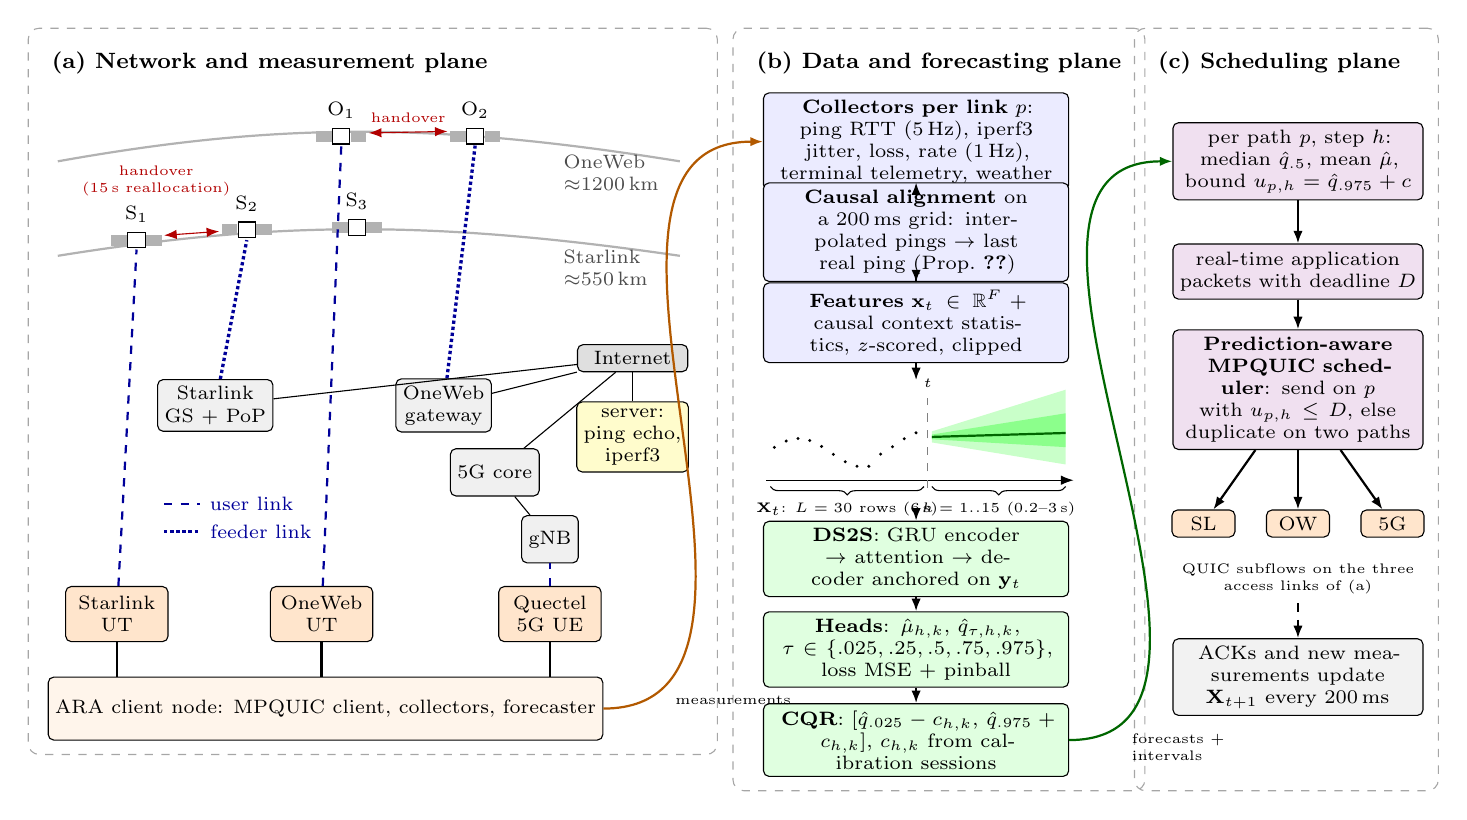
\begin{tikzpicture}[
  font=\scriptsize, >={Latex[length=1.6mm]},
  sat/.pic={\fill[gray!60] (-0.32,-0.07) rectangle (-0.12,0.07); \fill[gray!60] (0.12,-0.07) rectangle (0.32,0.07);
            \filldraw[fill=white, draw=black] (-0.11,-0.1) rectangle (0.11,0.1);},
  box/.style={draw, rounded corners=2pt, align=center, inner sep=2.5pt},
  gnd/.style={box, fill=gray!12, minimum height=6mm},
  ue/.style={box, fill=orange!20, minimum width=13mm, minimum height=7mm},
  pstep/.style={box, fill=blue!8, text width=37mm, minimum height=7mm},
  fstep/.style={box, fill=green!12, text width=37mm, minimum height=7mm},
  sch/.style={box, fill=violet!12, text width=30mm, minimum height=7mm},
  panel/.style={draw=gray!70, dashed, rounded corners=4pt, inner sep=5pt},
  ptitle/.style={font=\footnotesize\bfseries},
  ul/.style={dashed, thick, blue!60!black},
  fl/.style={densely dotted, very thick, blue!60!black},
  wl/.style={thick, ->}
]
% ===================== (a) network and measurement plane =====================
\node[ptitle, anchor=west] (ta) at (-0.5,8.75) {(a) Network and measurement plane};
\draw[gray!60, thick] (-0.3,6.3) .. controls (2.5,6.75) and (4.5,6.75) .. (7.6,6.3);
\draw[gray!60, thick] (-0.3,7.5) .. controls (2.5,8.0) and (4.5,8.0) .. (7.6,7.5);
\node[gray!60!black, anchor=west, align=left] at (6.0,6.15) {Starlink\\$\approx$550\,km};
\node[gray!60!black, anchor=west, align=left] at (6.0,7.35) {OneWeb\\$\approx$1200\,km};
\pic at (0.7,6.5) {sat}; \pic at (2.1,6.63) {sat}; \pic at (3.5,6.66) {sat};
\pic at (3.3,7.82) {sat}; \pic at (5.0,7.82) {sat};
\node at (0.7,6.83) {S$_1$}; \node at (2.1,6.96) {S$_2$}; \node at (3.5,6.99) {S$_3$};
\node at (3.3,8.15) {O$_1$}; \node at (5.0,8.15) {O$_2$};
\draw[<->, red!70!black] (1.05,6.56) -- (1.75,6.61);
\node[red!70!black, font=\tiny, align=center] at (0.95,7.25) {handover\\(15\,s reallocation)};
\draw[<->, red!70!black] (3.65,7.86) -- (4.65,7.88) node[midway, above, font=\tiny] {handover};
% ground segment
\node[gnd] (gs) at (1.7,4.4) {Starlink\\GS + PoP};
\node[gnd] (gw) at (4.6,4.4) {OneWeb\\gateway};
\node[gnd] (core) at (5.25,3.55) {5G core};
\node[box, fill=gray!25, minimum width=14mm] (inet) at (7.0,5.0) {Internet};
\node[box, fill=yellow!20] (srv) at (7.0,4.0) {server:\\ping echo,\\iperf3};
\draw[fl] (gs) -- (2.1,6.5);
\draw[fl] (gw) -- (5.0,7.7);
\draw (gs) -- (inet); \draw (gw) -- (inet); \draw (core) -- (inet); \draw (inet) -- (srv);
% user side
\node[ue] (sut) at (0.45,1.75) {Starlink\\UT};
\node[ue] (out) at (3.05,1.75) {OneWeb\\UT};
\node[ue] (qe) at (5.95,1.75) {Quectel\\5G UE};
\node[gnd] (gnb) at (5.95,2.7) {gNB};
\draw[ul] (sut) -- (0.7,6.38);
\draw[ul] (out) -- (3.3,7.7);
\draw[ul] (qe) -- (gnb); \draw (gnb) -- (core);
\node[box, fill=orange!8, minimum width=70mm, minimum height=8mm] (cn) at (3.1,0.55) {ARA client node: MPQUIC client, collectors, forecaster};
\draw[thick] (sut) -- (sut |- cn.north); \draw[thick] (out) -- (out |- cn.north); \draw[thick] (qe) -- (qe |- cn.north);
\draw[ul] (1.05,3.15) -- (1.5,3.15) node[right] {user link};
\draw[fl] (1.05,2.8) -- (1.5,2.8) node[right] {feeder link};
\node[panel, fit={(ta)(cn)(srv)(sut)(7.9,8.2)}] {};

% ===================== (b) data and forecasting plane =====================
\node[ptitle, anchor=west] (tb) at (8.45,8.75) {(b) Data and forecasting plane};
\node[pstep] (col) at (10.6,7.75) {\textbf{Collectors per link $p$}: ping RTT (5\,Hz), iperf3 jitter, loss, rate (1\,Hz), terminal telemetry, weather};
\node[pstep] (ali) at (10.6,6.6) {\textbf{Causal alignment} on a 200\,ms grid: interpolated pings $\rightarrow$ last real ping (Prop.~\ref{prop:leak})};
\node[pstep] (feat) at (10.6,5.45) {\textbf{Features} $\mathbf{x}_t\in\mathbb{R}^F$ + causal context statistics, $z$-scored, clipped};
\begin{scope}[shift={(8.7,3.45)}]
  \draw[->] (0,0) -- (3.9,0);
  \foreach \x in {0.1,0.25,...,2.0} \fill[black] (\x,{0.35+0.18*sin(220*\x)+0.1*(\x>1.3)}) circle (0.6pt);
  \draw[decorate, decoration={brace, amplitude=3pt, mirror}] (0.05,-0.08) -- (2.0,-0.08) node[midway, below=2pt, font=\tiny] {$\mathbf{X}_t$: $L=30$ rows (6\,s)};
  \draw[dashed, gray] (2.05,-0.1) -- (2.05,1.05) node[above, font=\tiny, black] {$t$};
  \fill[green!30, opacity=0.7] (2.1,0.48) -- (3.8,0.2) -- (3.8,1.15) -- (2.1,0.62) -- cycle;
  \fill[green!55, opacity=0.7] (2.1,0.52) -- (3.8,0.42) -- (3.8,0.85) -- (2.1,0.58) -- cycle;
  \draw[green!40!black, thick] (2.1,0.55) -- (3.8,0.6);
  \draw[decorate, decoration={brace, amplitude=3pt, mirror}] (2.1,-0.08) -- (3.8,-0.08) node[midway, below=2pt, font=\tiny] {$h=1..15$ (0.2--3\,s)};
\end{scope}
\node[fstep] (enc) at (10.6,2.45) {\textbf{DS2S}: GRU encoder $\rightarrow$ attention $\rightarrow$ decoder anchored on $\mathbf{y}_t$};
\node[fstep] (head) at (10.6,1.3) {\textbf{Heads}: $\hat\mu_{h,k}$, $\hat q_{\tau,h,k}$, $\tau\in\{.025,.25,.5,.75,.975\}$, loss MSE + pinball};
\node[fstep] (cqr) at (10.6,0.15) {\textbf{CQR}: $[\hat q_{.025}-c_{h,k},\,\hat q_{.975}+c_{h,k}]$, $c_{h,k}$ from calibration sessions};
\draw[wl] (col) -- (ali); \draw[wl] (ali) -- (feat); \draw[wl] (feat) -- (10.6,4.72); \draw[wl] (10.6,3.05) -- (enc);
\draw[wl] (enc) -- (head); \draw[wl] (head) -- (cqr);
\node[panel, fit={(tb)(col)(cqr)(8.55,3.0)(12.65,3.0)}] {};
\draw[wl, orange!70!black] (cn.east) to[out=0, in=180] node[pos=0.12, below right, font=\tiny, black] {measurements} (col.west);

% ===================== (c) scheduling plane =====================
\node[ptitle, anchor=west] (tc) at (13.55,8.75) {(c) Scheduling plane};
\node[sch] (fc) at (15.45,7.5) {per path $p$, step $h$: median $\hat q_{.5}$, mean $\hat\mu$, bound $u_{p,h}=\hat q_{.975}+c$};
\node[sch] (app) at (15.45,6.1) {real-time application packets with deadline $D$};
\node[sch] (dec) at (15.45,4.6) {\textbf{Prediction-aware MPQUIC scheduler}: send on $p$ with $u_{p,h}\le D$, else duplicate on two paths};
\node[box, fill=orange!20, minimum width=8mm] (p1) at (14.25,2.9) {SL};
\node[box, fill=orange!20, minimum width=8mm] (p2) at (15.45,2.9) {OW};
\node[box, fill=orange!20, minimum width=8mm] (p3) at (16.65,2.9) {5G};
\draw[wl] (fc) -- (app); \draw[wl] (app) -- (dec);
\draw[wl] (dec) -- (p1); \draw[wl] (dec) -- (p2); \draw[wl] (dec) -- (p3);
\node[align=center, font=\tiny] (sf) at (15.45,2.2) {QUIC subflows on the three\\access links of (a)};
\node[sch, fill=gray!10] (fb) at (15.45,0.95) {ACKs and new measurements update $\mathbf{X}_{t+1}$ every 200\,ms};
\draw[wl, dashed] (sf) -- (fb);
\node[panel, fit={(tc)(fc)(fb)(p1)(p3)(cqr.south -| fb.south)}] {};
\draw[wl, green!40!black] (cqr.east) to[out=0, in=180] node[pos=0.1, below right, font=\tiny, black, align=left] {forecasts +\\intervals} (fc.west);
\end{tikzpicture}
}
  \caption{System model. (a) A client node on the ARA living lab reaches a measurement server over three access links: a Starlink user terminal (UT) served by a shell at about 550\,km that reallocates users every 15\,s, a OneWeb UT served by a bent-pipe shell at about 1200\,km, and a 5G user equipment (UE). Handovers change the path RTT. (b) Per link, the collectors are aligned causally on a 200\,ms grid, and a window of 30 rows feeds the distributional forecaster (DS2S), whose quantiles are calibrated with CQR on held-out sessions. (c) The per-path forecasts and calibrated upper bounds drive a prediction-aware MPQUIC scheduler, and new measurements update the window every 200\,ms.}
  \label{fig:system}
\end{figure*}

\subsection{Data Set}
Table~\ref{tab:data} summarizes the data. The campaign comprises \DataSessions{} sessions and \DataRows{} million rows, which is \DataHours{} hours of 5\,Hz measurements over \DataDaysOW{} days for OneWeb and \DataDaysSL{} and \DataDaysQ{} days for Starlink and 5G. Sessions are split at random into 70\% training, 15\% calibration, and 15\% test sessions with a fixed seed. All windows of a session therefore stay in one set, and no test session is seen during training, model selection, or calibration. The OneWeb UL jitter and loss are zero in every row, and we report only RTT for that link. The 5G sets are about seven times larger than the satellite sets, and every fourth training window is used for all methods.

\begin{table}[t]
\centering
\caption{Data set. Rows are 200\,ms apart. A window has 30 input and 15 target rows. Features: base / extended input set.}
\label{tab:data}
\footnotesize
\setlength{\tabcolsep}{2.2pt}
\begin{tabular}{lrrrrrc}
\toprule
Link & Sessions & Hours & Train win. & Calib.\ win. & Test win. & Features \\
\midrule
OneWeb DL   & 45/9/11   & \DataHoursOWDL & 117{,}558 & 22{,}655  & 27{,}492  & 9/31 \\
OneWeb UL   & 45/9/11   & \DataHoursOWUL & 115{,}847 & 22{,}751  & 28{,}125  & 9/31 \\
Starlink DL & 37/7/9    & \DataHoursSLDL & 105{,}906 & 20{,}025  & 25{,}838  & 19/41 \\
Starlink UL & 37/7/9    & \DataHoursSLUL & 106{,}165 & 20{,}090  & 25{,}666  & 19/41 \\
5G DL       & 266/57/58 & \DataHoursQDL & 194{,}725 & 166{,}266 & 169{,}204 & 10/32 \\
5G UL       & 265/56/58 & \DataHoursQUL & 193{,}502 & 162{,}894 & 168{,}519 & 10/32 \\
\bottomrule
\end{tabular}
\end{table}

\subsection{Forecasting Problem}
For one link, let $\mathbf{x}_t\in\RR^{F}$ be the feature vector of row $t$ and $\mathbf{y}_t\in\RR^{K}$ the $K=3$ targets: RTT (ms), iperf jitter (ms), and iperf loss (\%). The targets are also part of $\mathbf{x}_t$. Given the window $\mathbf{X}_t=(\mathbf{x}_{t-L+1},\dots,\mathbf{x}_t)$ of $L=30$ rows (6\,s), the forecaster outputs, for every step $h\in\{1,\dots,H\}$ with $H=15$ (0.2--3\,s) and every target $k$, a point forecast and a $(1-\alpha)$ prediction interval $[\ell_{t,h,k},u_{t,h,k}]$.

A forecast is judged by a loss averaged over test windows. For point forecasts we use the squared and the absolute error. For a $(1-\alpha)$ interval we use the interval score~\cite{gneiting2007strictly}
\begin{equation}
\mathrm{IS}_\alpha(\ell,u;y)=(u-\ell)+\tfrac{2}{\alpha}(\ell-y)^{+}+\tfrac{2}{\alpha}(y-u)^{+},
\label{eq:is}
\end{equation}
with $(z)^+=\max\{z,0\}$. The score adds the width of the interval and a penalty proportional to the size of every miss, which is the trade-off a deadline-aware scheduler faces: a wide bound wastes capacity on redundancy, and a miss costs a late packet.

\begin{proposition}
\label{prop:optimal}
Let $Y$ be the target given the input window, with finite variance. The expected squared error is minimized by $\E[Y]$, the expected absolute error by any median of $Y$, and the expected pinball loss $\rho_\tau(Y-q)$ with $\rho_\tau(e)=\max\{\tau e,(\tau-1)e\}$ by any $\tau$-quantile of $Y$. The expected interval score~\eqref{eq:is} is minimized by $\ell=q_{\alpha/2}$ and $u=q_{1-\alpha/2}$.
\end{proposition}
\begin{IEEEproof}
These are standard results~\cite{gneiting2011making,koenker1978regression}. For the interval score, $\mathrm{IS}_\alpha(\ell,u;y)=\frac{2}{\alpha}\big[\rho_{\alpha/2}(y-\ell)+\rho_{1-\alpha/2}(y-u)\big]$, which can be checked case by case for $y<\ell$, $\ell\le y\le u$, and $y>u$. The two terms are minimized separately by the stated quantiles.
\end{IEEEproof}

Proposition~\ref{prop:optimal} has a direct consequence that guides the rest of the paper. The optimal interval follows the conditional quantiles of $Y$. Its width must therefore change with the input whenever the spread of $Y$ does. A model that outputs only a mean, wrapped in an interval of constant width, cannot be optimal if the spread varies, however accurate its mean is. Section~\ref{sec:predictable} shows that the spread of LEO link state varies strongly and predictably.

\section{What Is Predictable in Sub-Second Link State?}
\label{sec:predictable}
Before we build a forecaster, we ask which properties of the RTT carry over from the input window to the forecast horizon. The statistics in this section use the measured pings of the training sessions, with each session centered on its own mean so that differences between sessions do not appear as memory. Confidence intervals come from a bootstrap over sessions.

\begin{figure*}[t]
  \centering
  % fr_volatility.tex - data from modeling/experiments/fr_volatility.py (results_final/analysis/volatility/).
% Autocorrelation on TRAINING sessions of the RTT level, the RTT change dRTT and the change size |dRTT|,
% lags 0.2-10 s, pairs inside one session only, each session centred on its own mean, real pings only.
% Shaded bands: 95% session-bootstrap intervals. Insets zoom into the boxed region (lags up to 3 s, near zero)
% with the same range in every inset. Starlink DL has no inset: its 1 s sawtooth is visible at full scale.
% Open black circles at 0.2 s: the same ACF after shuffling the real pings inside every session (memoryless null).
% Where a curve starts on its circle, the first lag is mechanical (one spike = two large changes), not memory.
% Needs: \input{figs/data/plotstyle.tex}, pgfplots groupplots, tikz calc. No fillbetween library.
\begin{tikzpicture}
\tikzset{
  volZero/.style={black!65, line width=0.4pt},
  volBox/.style={black!70, line width=0.5pt},
  volArrow/.style={->, >=stealth, black!70, line width=0.5pt, shorten >=1pt},
}
\pgfplotsset{
  volL/.style={cPers, densely dashed, thick, mark=none},
  volD/.style={cResid, thick, mark=triangle*, mark size=1.5pt, mark indices={1,5,10,15,20,25,30,35,40,45,50}},
  volA/.style={cFR, very thick, mark=square*, mark size=1.1pt, mark indices={1,5,10,15,20,25,30,35,40,45,50}},
  volBandD/.style={draw=none, fill=cResid, fill opacity=0.28, forget plot},
  volBandA/.style={draw=none, fill=cFR, fill opacity=0.28, forget plot},
  volInset/.style={scale only axis, width=2.45cm, height=1.5cm, xmin=0.1, xmax=3.1, ymin=-0.15, ymax=0.3,
    xtick={0.2,1,2,3}, xticklabels={0.2,1,2,3}, ytick={-0.1,0,0.1,0.2,0.3}, yticklabels={,0,,0.2,},
    tick label style={font=\tiny}, axis background/.style={fill=white}, grid=major, grid style={gray!20},
    xticklabel style={fill=white, inner sep=0.5pt}, yticklabel style={fill=white, inner sep=0.5pt},
    clip=true},
  volInD/.style={cResid, thick, mark=triangle*, mark size=1.0pt},
  volInA/.style={cFR, thick, mark=square*, mark size=0.75pt},
  volNullMark/.style={only marks, mark=o, mark size=2.2pt, black, line width=0.6pt},
  volNull/.style={volNullMark, restrict x to domain=0:0.3, forget plot},
}
\begin{groupplot}[group style={group size=3 by 2, horizontal sep=0.32cm, vertical sep=0.9cm,
    y descriptions at=edge left, x descriptions at=edge bottom},
  frbase, scale only axis, width=5.05cm, height=3.3cm, xmin=0, xmax=10, ymin=-0.58, ymax=1.0,
  xtick={0,2,4,6,8,10}, ytick={-0.5,0,0.5,1}, xlabel={lag (s)}, ylabel={autocorrelation}]
% ---------------- (a) OneWeb DL
\nextgroupplot[title={(a) OneWeb DL}, legend to name=legvol, legend columns=-1,
  legend style={draw=black!60, fill=white, font=\scriptsize, /tikz/every even column/.append style={column sep=0.3cm}}]
\addplot[volBandD] table[x=x, y=d] {figs/data/fr_volatility_band_oneweb_dl.dat} -- cycle;
\addplot[volBandA] table[x=x, y=absd] {figs/data/fr_volatility_band_oneweb_dl.dat} -- cycle;
\draw[volZero] (axis cs:0,0) -- (axis cs:10,0);
\addplot[volL] table[x=lag_s, y=rtt] {figs/data/fr_volatility_acf_oneweb_dl.dat}; \addlegendentry{RTT level}
\addplot[volD] table[x=lag_s, y=d] {figs/data/fr_volatility_acf_oneweb_dl.dat}; \addlegendentry{RTT change $\Delta$RTT}
\addplot[volA] table[x=lag_s, y=absd] {figs/data/fr_volatility_acf_oneweb_dl.dat}; \addlegendentry{change size $|\Delta\mathrm{RTT}|$}
\addplot[volNull] table[x=lag_s, y=dnull] {figs/data/fr_volatility_acf_oneweb_dl.dat};
\addplot[volNull] table[x=lag_s, y=absdnull] {figs/data/fr_volatility_acf_oneweb_dl.dat};
\addlegendimage{area legend, draw=none, fill=black!22}\addlegendentry{95\% session bootstrap}
\addlegendimage{volNullMark}\addlegendentry{memoryless null}
\draw[volBox] (axis cs:0.1,-0.15) rectangle (axis cs:3.1,0.3);
\coordinate (zA) at (axis cs:3.1,0.3);
% ---------------- (b) Starlink DL (no inset)
\nextgroupplot[title={(b) Starlink DL}]
\addplot[volBandD] table[x=x, y=d] {figs/data/fr_volatility_band_starlink_dl.dat} -- cycle;
\addplot[volBandA] table[x=x, y=absd] {figs/data/fr_volatility_band_starlink_dl.dat} -- cycle;
\draw[volZero] (axis cs:0,0) -- (axis cs:10,0);
\addplot[volL] table[x=lag_s, y=rtt] {figs/data/fr_volatility_acf_starlink_dl.dat};
\addplot[volD] table[x=lag_s, y=d] {figs/data/fr_volatility_acf_starlink_dl.dat};
\addplot[volA] table[x=lag_s, y=absd] {figs/data/fr_volatility_acf_starlink_dl.dat};
\addplot[volNull] table[x=lag_s, y=dnull] {figs/data/fr_volatility_acf_starlink_dl.dat};
\addplot[volNull] table[x=lag_s, y=absdnull] {figs/data/fr_volatility_acf_starlink_dl.dat};
\node[font=\scriptsize, fill=white, inner sep=1.5pt, anchor=north east] at (axis cs:9.8,0.97) {peaks every 1 s};
% ---------------- (c) 5G DL
\nextgroupplot[title={(c) 5G DL}]
\addplot[volBandD] table[x=x, y=d] {figs/data/fr_volatility_band_quectel_dl.dat} -- cycle;
\addplot[volBandA] table[x=x, y=absd] {figs/data/fr_volatility_band_quectel_dl.dat} -- cycle;
\draw[volZero] (axis cs:0,0) -- (axis cs:10,0);
\addplot[volL] table[x=lag_s, y=rtt] {figs/data/fr_volatility_acf_quectel_dl.dat};
\addplot[volD] table[x=lag_s, y=d] {figs/data/fr_volatility_acf_quectel_dl.dat};
\addplot[volA] table[x=lag_s, y=absd] {figs/data/fr_volatility_acf_quectel_dl.dat};
\addplot[volNull] table[x=lag_s, y=dnull] {figs/data/fr_volatility_acf_quectel_dl.dat};
\addplot[volNull] table[x=lag_s, y=absdnull] {figs/data/fr_volatility_acf_quectel_dl.dat};
\draw[volBox] (axis cs:0.1,-0.15) rectangle (axis cs:3.1,0.3);
\coordinate (zC) at (axis cs:3.1,0.3);
% ---------------- (d) OneWeb UL
\nextgroupplot[title={(d) OneWeb UL}]
\addplot[volBandD] table[x=x, y=d] {figs/data/fr_volatility_band_oneweb_ul.dat} -- cycle;
\addplot[volBandA] table[x=x, y=absd] {figs/data/fr_volatility_band_oneweb_ul.dat} -- cycle;
\draw[volZero] (axis cs:0,0) -- (axis cs:10,0);
\addplot[volL] table[x=lag_s, y=rtt] {figs/data/fr_volatility_acf_oneweb_ul.dat};
\addplot[volD] table[x=lag_s, y=d] {figs/data/fr_volatility_acf_oneweb_ul.dat};
\addplot[volA] table[x=lag_s, y=absd] {figs/data/fr_volatility_acf_oneweb_ul.dat};
\addplot[volNull] table[x=lag_s, y=dnull] {figs/data/fr_volatility_acf_oneweb_ul.dat};
\addplot[volNull] table[x=lag_s, y=absdnull] {figs/data/fr_volatility_acf_oneweb_ul.dat};
\draw[volBox] (axis cs:0.1,-0.15) rectangle (axis cs:3.1,0.3);
\coordinate (zD) at (axis cs:3.1,0.3);
% ---------------- (e) Starlink UL
\nextgroupplot[title={(e) Starlink UL}]
\addplot[volBandD] table[x=x, y=d] {figs/data/fr_volatility_band_starlink_ul.dat} -- cycle;
\addplot[volBandA] table[x=x, y=absd] {figs/data/fr_volatility_band_starlink_ul.dat} -- cycle;
\draw[volZero] (axis cs:0,0) -- (axis cs:10,0);
\addplot[volL] table[x=lag_s, y=rtt] {figs/data/fr_volatility_acf_starlink_ul.dat};
\addplot[volD] table[x=lag_s, y=d] {figs/data/fr_volatility_acf_starlink_ul.dat};
\addplot[volA] table[x=lag_s, y=absd] {figs/data/fr_volatility_acf_starlink_ul.dat};
\addplot[volNull] table[x=lag_s, y=dnull] {figs/data/fr_volatility_acf_starlink_ul.dat};
\addplot[volNull] table[x=lag_s, y=absdnull] {figs/data/fr_volatility_acf_starlink_ul.dat};
\draw[volBox] (axis cs:0.1,-0.15) rectangle (axis cs:3.1,0.3);
\coordinate (zE) at (axis cs:3.1,0.3);
% ---------------- (f) 5G UL
\nextgroupplot[title={(f) 5G UL}]
\addplot[volBandD] table[x=x, y=d] {figs/data/fr_volatility_band_quectel_ul.dat} -- cycle;
\addplot[volBandA] table[x=x, y=absd] {figs/data/fr_volatility_band_quectel_ul.dat} -- cycle;
\draw[volZero] (axis cs:0,0) -- (axis cs:10,0);
\addplot[volL] table[x=lag_s, y=rtt] {figs/data/fr_volatility_acf_quectel_ul.dat};
\addplot[volD] table[x=lag_s, y=d] {figs/data/fr_volatility_acf_quectel_ul.dat};
\addplot[volA] table[x=lag_s, y=absd] {figs/data/fr_volatility_acf_quectel_ul.dat};
\addplot[volNull] table[x=lag_s, y=dnull] {figs/data/fr_volatility_acf_quectel_ul.dat};
\addplot[volNull] table[x=lag_s, y=absdnull] {figs/data/fr_volatility_acf_quectel_ul.dat};
\draw[volBox] (axis cs:0.1,-0.15) rectangle (axis cs:3.1,0.3);
\coordinate (zF) at (axis cs:3.1,0.3);
\end{groupplot}
% ---------------- insets: lags up to 3 s near zero, same range in every inset
\foreach \g/\c/\ds in {A/c1r1/oneweb_dl, C/c3r1/quectel_dl, D/c1r2/oneweb_ul, E/c2r2/starlink_ul, F/c3r2/quectel_ul}{
  \begin{axis}[volInset, at={($(group \c.north east)+(-0.1cm,-0.12cm)$)}, anchor=north east, name=ins\g]
  \addplot[volBandD] table[x=x, y=d] {figs/data/fr_volatility_band_\ds.dat} -- cycle;
  \addplot[volBandA] table[x=x, y=absd] {figs/data/fr_volatility_band_\ds.dat} -- cycle;
  \draw[volZero] (axis cs:0,0) -- (axis cs:3.2,0);
  \addplot[volInD] table[x=lag_s, y=d] {figs/data/fr_volatility_acf_\ds.dat};
  \addplot[volInA] table[x=lag_s, y=absd] {figs/data/fr_volatility_acf_\ds.dat};
  \end{axis}
  \draw[volArrow] (z\g) -- (ins\g.south west);
}
\node at ($(group c2r1.north)+(0,0.8cm)$) {\pgfplotslegendfromname{legvol}};
\end{tikzpicture}

  \caption{Autocorrelation of the RTT level, of its 200\,ms change $\Delta$RTT, and of the size of the change $|\Delta\mathrm{RTT}|$ in the training sessions (shaded: 95\% session-bootstrap interval). Circles: value of a memoryless series at 0.2\,s. A curve that starts on its circle has no memory at the first lag. Insets: lags of 0.2 to 3\,s. Starlink DL peaks every second because of a load-driven sawtooth.}
  \label{fig:vol}
\end{figure*}

\subsection{The Next Change Is Hard, the Level Reverts}
Fig.~\ref{fig:vol} shows the autocorrelation of the RTT level, of its change $\Delta$RTT between consecutive rows, and of the size of the change $|\Delta\mathrm{RTT}|$. At the first lag, the change of a memoryless series has an autocorrelation of $-0.5$ (circles), because two consecutive changes share one sample. From 0.4\,s to 10\,s the autocorrelation of $\Delta$RTT stays within $\pm$\VolDmaxAbs{} on five links. Past changes therefore say almost nothing about the next change. This does not make the direction of the next change unpredictable, because the RTT returns toward its recent level. Expecting a return to the mean of the 6\,s input window gets the sign of the 1\,s change right in \VolSignRevLo\% to \VolSignRevHi\% of the test windows (balanced accuracy, 50\% for a constant guess), and the learned forecasters of Section~\ref{sec:results} reach \VolSignNNLo\% to \VolSignNNHi\%. Point forecasts thus beat persistence mainly by not repeating the last, noisy ping. Scaled by the error of persistence, a common reference for forecast accuracy~\cite{hyndman2006another}, their MAE is \PersRatioLo{} to \PersRatioHi{} times lower.

\subsection{The Spread Depends on the Link State}
The size of the change has a short memory. The autocorrelation of $|\Delta\mathrm{RTT}|$ at 1\,s is \VolAbsdLo{} to \VolAbsdHi{} on OneWeb and 5G DL, and on the five links without a sawtooth it stays positive for 1.4 to 5.8\,s. Inside a session, this memory is too weak to forecast the next seconds. On OneWeb and 5G, the standard deviation (SD) of the 6\,s input does not predict the error of a 1\,s forecast within a session (rank correlation \VolWithinLo{} to \VolWithinHi), but it does between sessions (\VolBetweenLo{} to \VolBetweenHi). Each session runs in a noise regime set by its load and radio conditions, and a few seconds of input reveal the regime. Starlink DL also has dynamics within a session. Under the saturating downlink test, its RTT climbs from about 35\,ms to about 200\,ms in steps of about 50\,ms and drops back once per second, which produces the peaks of Fig.~\ref{fig:vol}(b). The RTT autocorrelation at 1\,s is \VolSLDLlevel{} and exceeds \VolSLDLlevelMin{} in every one of the \VolSLDLnSess{} training sessions. The sawtooth switches on and off within a session, as in Fig.~\ref{fig:trace}, and the volatility of the last 6\,s predicts that of the next 3\,s (within-session rank correlation \VolSLDLrv). We attribute the sawtooth to queue build-up and drain under the saturating load, since the uplink test does not show it.

\subsection{Errors Are Skewed Upward}
The RTT also moves up further than it moves down. Queues and retransmissions add delay, while nothing removes delay below the propagation floor. For the 1\,s forecasts of the previous model, the 97.5\% quantile of the error on the calibration sessions is \SkewQUL{} times the size of the 2.5\% quantile on 5G UL and \SkewOWDL{} times on OneWeb DL. A symmetric interval around a point forecast wastes width below the forecast.

\subsection{Consequence for Uncertainty}
An interval of constant width around a point forecast ignores both properties. Calibrated to cover 95\% of all windows, it covers \CovConstCalmLo{} to \CovConstCalmHi{} of the calmest tenth of windows, ranked by the input SD, and \CovConstVolLo{} to \CovConstVolHi{} of the most volatile tenth. The calm windows are covered more often on every link. On Starlink DL the interval is \WidConstSLDL\,ms wide at 1\,s ahead in every window, while a quiet window rarely moves by more than a few milliseconds. By Proposition~\ref{prop:optimal}, the optimal interval follows the conditional quantiles. A forecaster should therefore learn the spread and its skew from the input. Because the regime differs between sessions, its intervals must be calibrated on sessions that it has not seen.

\section{Causality of the Measurement Pipeline}
\label{sec:causal}
The collectors run on independent clocks. When a ping is missing at row $t$, a common merging step fills it by time interpolation between the neighboring real pings. Let $y_{t-1}$ and $y_{t+1}$ be the real pings around a single missing row and let the parser write $\tilde{y}_t=(1-w)\,y_{t-1}+w\,y_{t+1}$, with $w\in(0,1)$ the relative time position of row $t$ ($w=1/2$ for evenly spaced rows). The forecast origin $\tilde{y}_t$ then contains part of the first target $y_{t+1}$.

\begin{proposition}
\label{prop:leak}
For a window whose last row is interpolated as above, the one-step persistence error with the interpolated origin is $y_{t+1}-\tilde{y}_t=(1-w)\,(y_{t+1}-y_{t-1})$, which is $(1-w)$ times the error with the causal origin $y_{t-1}$. Its squared error is therefore $(1-w)^2$ times the causal one for any realization of the process, a factor of four for $w=1/2$. If a fraction $p$ of the windows have an interpolated origin with $w=1/2$, and the causal one-step errors of these windows have the same mean square as the others, the one-step RMSE of persistence is understated by the factor $\sqrt{1-3p/4}$.
\end{proposition}
\begin{IEEEproof}
Substitute $\tilde{y}_t$ into $y_{t+1}-\tilde{y}_t$ for the first statement. For the second, the mean squared error over all windows is $(1-p)\,m+p\,m/4=m(1-3p/4)$, where $m$ is the causal mean squared error.
\end{IEEEproof}

In our Starlink DL data, \InterpFracSLDL\% of the test RTT samples are interpolated. Replacing every interpolated input by the last real ping raises the one-step persistence RMSE by \AuditPersHonePct\%, from \AuditPersLegacyHone{} to \AuditPersCausalHone\,ms. This is more than the 5\% that Proposition~\ref{prop:leak} predicts under equal errors, because the windows with an interpolated origin have larger one-step errors than the others. The 5G and OneWeb RTT series contain no interpolated values.

\begin{figure}[t]
  \centering
  % fr_leak.tex - generated by modeling/experiments/fr_leak.py, do not edit by hand.
\begin{tikzpicture}
\begin{axis}[frbase, name=main, width=8.7cm, height=5.4cm, xmin=0.2, xmax=3, xtick={0.2,1,2,3}, ymin=13, ymax=26,
  xlabel={horizon (s)}, ylabel={DS2S RTT MAE (ms), Starlink DL}, legend cell align=left,
  legend style={at={(0.5,1.03)}, anchor=south, legend columns=1, font=\scriptsize, draw=none}]
\addplot[cPrev, thick, mark=o, mark size=1.2pt] table[x=t, y=A_leak_leak] {figs/data/fr_leak_DS2S_MAE.dat}; \addlegendentry{interpolated train and test (reported)}
\addplot[cResid, thick, dashed, mark=triangle*, mark size=1.3pt] table[x=t, y=B_leak_causal] {figs/data/fr_leak_DS2S_MAE.dat}; \addlegendentry{interpolated train, causal test (deployed)}
\addplot[cFR, very thick, mark=square*, mark size=1.1pt] table[x=t, y=C_causal_causal] {figs/data/fr_leak_DS2S_MAE.dat}; \addlegendentry{causal train and test (this paper)}
\draw[black!70] (axis cs:0.2,14.19) rectangle (axis cs:0.6,18.41);
\coordinate (lz) at (axis cs:0.6,16.3);
\end{axis}
\begin{axis}[at={($(main.south east)+(-0.2cm,0.5cm)$)}, anchor=south east, width=3.4cm, height=2.6cm, xmin=0.2, xmax=0.6,
  ymin=14.19, ymax=18.41, xtick={0.2,0.4,0.6}, tick label style={font=\tiny}, axis background/.style={fill=white}, grid=major, grid style={gray!20}, name=ins]
\addplot[cPrev, thick, mark=o, mark size=1pt] table[x=t, y=A_leak_leak] {figs/data/fr_leak_DS2S_MAE.dat};
\addplot[cResid, thick, dashed, mark=triangle*, mark size=1pt] table[x=t, y=B_leak_causal] {figs/data/fr_leak_DS2S_MAE.dat};
\addplot[cFR, very thick, mark=square*, mark size=1pt] table[x=t, y=C_causal_causal] {figs/data/fr_leak_DS2S_MAE.dat};
\end{axis}
\draw[->, black!70] (lz) -- (ins.west);
\end{tikzpicture}

  \caption{Effect of the interpolation leak on a trained forecaster (DS2S, Starlink DL, mean of three seeds). Trained and tested on interpolated inputs, the model reports a lower error than it reaches when it is deployed on the causal inputs available online. Inset: the first 0.6\,s.}
  \label{fig:leak}
\end{figure}

The leak is not limited to persistence. Every model that reads the last input value, including anchored decoders and rolling features, can exploit it. Fig.~\ref{fig:leak} measures the effect on a trained model. We trained S2S and DS2S of Section~\ref{sec:setup} on Starlink DL with interpolated inputs and, separately, with causal inputs that hold the last real ping, three seeds each, and tested the models trained on interpolated inputs on both versions of the test inputs. The targets are the same measured series in all cases. Trained and tested on interpolated inputs, DS2S reports a 0.2\,s MAE of \LeakDSAhOne\,ms. On causal inputs, which are all that a deployed forecaster sees, the same model reaches \LeakDSBhOne\,ms, \LeakOptDSMAEhOne\% worse (RMSE: \LeakOptDSRMSEhOne\%). The model trained on causal inputs reaches \LeakDSChOne\,ms. Causal training thus also gives the better deployed model. The gap shrinks with the horizon (\LeakOptDSMAEavg\% over 0.2 to 3\,s) and is smaller for S2S (\LeakOptSSMAEhOne\% at 0.2\,s), whose decoder does not start from the last observation. The leak therefore inflates the short-horizon accuracy on which a packet scheduler relies most. All other results in this paper use causal inputs and measured targets.

\section{Distributional Forecaster with Conformal Calibration}
\label{sec:method}
\subsection{Encoder and Attention}
Fig.~\ref{fig:arch} shows the forecaster. Each input row is concatenated with a learned embedding of the sine and cosine of the hour of day and the day of week, and a two-layer GRU encoder with hidden size $d=128$~\cite{cho2014learning} maps the window to the states $\mathbf{e}_{t-L+1},\dots,\mathbf{e}_t$. At decoder step $h$ the additive attention~\cite{bahdanau2015neural} forms the context $\mathbf{c}_h=\sum_{j}a_{h,j}\mathbf{e}_j$ with $a_{h,j}\propto\exp\big(\mathbf{v}^\top\tanh(\mathbf{W}_q\mathbf{s}_{h-1}+\mathbf{W}_k\mathbf{e}_j)\big)$, where $\mathbf{s}_{h-1}$ is the top decoder state. The encoder and the attention are those of the baseline. The comparison therefore isolates the decoder and the output.

\begin{figure}[t]
  \centering
  \resizebox{\columnwidth}{!}{% Year 3 forecaster: GRU encoder, additive attention, residual autoregressive decoder.
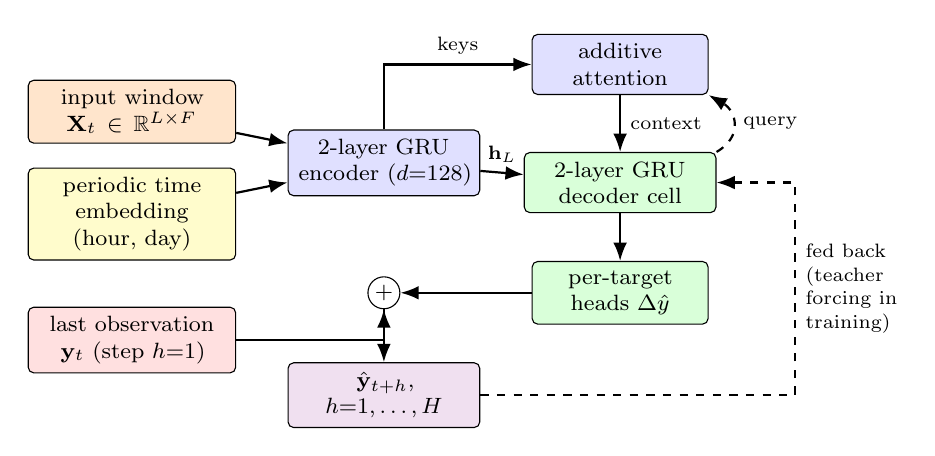
\begin{tikzpicture}[
  font=\footnotesize, >=Latex,
  b/.style={draw, rounded corners=2pt, minimum height=7mm, align=center, fill=#1},
  b/.default=gray!10,
  lnk/.style={->, thick}
]
\node[b=orange!20, text width=24mm] (in) at (0,0) {input window\\$\mathbf{X}_t\in\mathbb{R}^{L\times F}$};
\node[b=yellow!20, text width=24mm] (te) at (0,-1.3) {periodic time\\embedding (hour, day)};
\node[b=blue!12, text width=22mm] (enc) at (3.2,-0.65) {2-layer GRU\\encoder ($d{=}128$)};
\node[b=blue!12, text width=20mm] (att) at (6.2,0.6) {additive\\attention};
\node[b=green!15, text width=22mm] (dec) at (6.2,-0.9) {2-layer GRU\\decoder cell};
\node[b=green!15, text width=20mm] (head) at (6.2,-2.3) {per-target\\heads $\Delta\hat{y}$};
\node[draw, circle, inner sep=1pt, fill=white] (sum) at (3.2,-2.3) {$+$};
\node[b=red!12, text width=24mm] (last) at (0,-2.9) {last observation\\$\mathbf{y}_t$ (step $h{=}1$)};
\node[b=violet!12, text width=22mm] (out) at (3.2,-3.6) {$\hat{\mathbf{y}}_{t+h}$, $h{=}1,\dots,H$};
\draw[lnk] (in) -- (enc);
\draw[lnk] (te) -- (enc);
\draw[lnk] (enc) |- node[pos=0.75, above]{\scriptsize keys} (att);
\draw[lnk] (enc) -- node[above]{\scriptsize $\mathbf{h}_L$} (dec);
\draw[lnk] (att) -- node[right]{\scriptsize context} (dec);
\draw[lnk] (dec) -- (head);
\draw[lnk] (head) -- (sum);
\draw[lnk] (last) -| (sum);
\draw[lnk] (sum) -- (out);
\draw[lnk, dashed] (out.east) -| ++(4.0,0) |- node[pos=0.25, right, align=left]{\scriptsize fed back\\[-1pt]\scriptsize (teacher\\[-1pt]\scriptsize forcing in\\[-1pt]\scriptsize training)} (dec.east);
\draw[lnk, dashed] (dec.north east) to[out=30, in=-30, looseness=1.4] node[right]{\scriptsize query} (att.south east);
\end{tikzpicture}
}
  \caption{Proposed forecaster. The decoder is anchored on the last observation, and each head outputs a mean and five non-crossing quantiles of the change.}
  \label{fig:arch}
\end{figure}

\subsection{Anchored Distributional Decoder}
A two-layer GRU decoder cell takes $\mathbf{c}_h$ and an embedding of the previous mean forecast $\hat{\boldsymbol{\mu}}_{t+h-1}$, with $\hat{\boldsymbol{\mu}}_{t}=\mathbf{y}_t$ read from the input window, and produces $\mathbf{s}_h$. For each target $k$ a head $g_k$ (a two-layer perceptron) outputs six numbers $(m,r,a_1,a_2,b_1,b_2)$, from which
\begin{align}
\hat{\mu}_{t+h,k}&=\hat{\mu}_{t+h-1,k}+m, \qquad \hat{q}_{0.5}=\hat{\mu}_{t+h-1,k}+r,\label{eq:anchor}\\
\hat{q}_{0.25}&=\hat{q}_{0.5}-\varsigma(a_1),\quad \hat{q}_{0.025}=\hat{q}_{0.25}-\varsigma(a_2),\nonumber\\
\hat{q}_{0.75}&=\hat{q}_{0.5}+\varsigma(b_1),\quad \hat{q}_{0.975}=\hat{q}_{0.75}+\varsigma(b_2),\nonumber
\end{align}
with $\varsigma(z)=\log(1+e^{z})+\epsilon$ and $\epsilon=10^{-4}$. The anchoring in~\eqref{eq:anchor} makes persistence the forecast obtained when all head outputs are zero. The network only learns departures from the last value. Because $\varsigma>0$, the five quantiles are strictly ordered for every input, which removes the quantile crossing that separate quantile heads can produce. The decoder feeds back the mean, which keeps the recursion identical to the baseline.

\subsection{Training Loss}
With targets normalized by training statistics, the loss over a batch of $N$ windows is
\begin{equation}
\mathcal{L}=\frac{1}{NHK}\sum_{n,h,k}\Big[(\hat{\mu}_{nhk}-y_{nhk})^2+\frac{1}{5}\sum_{\tau\in\mathcal{T}}\rho_\tau(y_{nhk}-\hat{q}_{\tau,nhk})\Big],
\label{eq:loss}
\end{equation}
with $\mathcal{T}=\{0.025,0.25,0.5,0.75,0.975\}$. By Proposition~\ref{prop:optimal}, the population minimizer of~\eqref{eq:loss} over unrestricted functions of the window is the conditional mean for $\hat{\mu}$ and the conditional $\tau$-quantile for each $\hat{q}_\tau$. These targets are compatible with the ordering constraint, since conditional quantiles are ordered. The point forecast reported for squared-error metrics is $\hat{\mu}$ and for absolute-error metrics $\hat{q}_{0.5}$. Teacher forcing is applied per sample with a probability that decays from 0.5 to 0 over half of the epochs~\cite{bengio2015scheduled}.

\subsection{Conformal Calibration Across Sessions}
The learned quantiles are fitted on training sessions and may under-cover or over-cover new sessions. Let $\mathcal{C}$ be the windows of the calibration sessions and, for each step $h$ and target $k$, define the CQR score~\cite{romano2019conformalized}
\begin{equation}
s_i=\max\{\hat{q}_{\alpha/2}(\mathbf{X}_i)-y_i,\;y_i-\hat{q}_{1-\alpha/2}(\mathbf{X}_i)\},\qquad i\in\mathcal{C}.
\end{equation}
With $c_{h,k}$ the $\lceil(|\mathcal{C}|+1)(1-\alpha)\rceil$-th smallest score, the interval is $[\hat{q}_{\alpha/2}-c_{h,k},\,\hat{q}_{1-\alpha/2}+c_{h,k}]$. If the calibration and test windows are exchangeable, its coverage is at least $1-\alpha$~\cite{romano2019conformalized}. Windows of one session overlap and sessions differ in time of day and load. Exchangeability therefore holds only approximately~\cite{barber2023conformal}, and we report the coverage measured on test sessions. For a model without quantiles we use the split conformal interval $\hat{y}\pm c$ with $c$ the same order statistic of $|y_i-\hat{y}_i|$~\cite{lei2018distribution}.

\subsection{Seed Ensembles and Complexity}
Three models trained with different seeds are combined by averaging their mean and each quantile, which keeps the ordering, and the ensemble is calibrated in the same way~\cite{lakshminarayanan2017simple}. The forecaster has \ParamsDist{} parameters against \ParamsYtwo{} for the scalar baseline on OneWeb DL. A forecast needs one encoder pass and $H$ decoder steps, as in the baseline. Algorithm~\ref{alg:cqr} summarizes training, calibration, and inference.

\begin{algorithm}[t]
\caption{Training, calibration, and online use}
\label{alg:cqr}
\begin{algorithmic}[1]
\REQUIRE training, calibration, and test sessions, $\alpha$, seeds $\mathcal{S}$
\FOR{each seed in $\mathcal{S}$}
  \STATE train the forecaster with~\eqref{eq:loss} on training sessions, select the checkpoint with the lowest smoothed calibration-session loss
\ENDFOR
\STATE average the means and quantiles of the seeds
\FOR{each step $h$ and target $k$}
  \STATE compute the CQR scores on calibration windows and the offset $c_{h,k}$
\ENDFOR
\STATE \textbf{online:} for a new window, output $\hat{\mu}$, $\hat{q}_{0.5}$, and $[\hat{q}_{\alpha/2}-c_{h,k},\hat{q}_{1-\alpha/2}+c_{h,k}]$ for all $h,k$
\end{algorithmic}
\end{algorithm}

\section{Evaluation Setup}
\label{sec:setup}
\subsection{Inputs}
The base feature set of each link (left number in the last column of Table~\ref{tab:data}) holds the three targets, the iperf throughput, the link telemetry listed in Section~\ref{sec:system}, and for Starlink and 5G three weather variables. The extended set adds, for each target, seven causal statistics computed within the session: the number of rows since the value last changed (the phase in the report cycle, since jitter and loss are one-second reports held for five rows), the mean and maximum of the last second, the means of the last 30\,s and 60\,s, the standard deviation of the last 60\,s, and the session-to-date mean. It also adds the time since the previous row. Radio values outside physical ranges, such as the logger sentinel $-32768$ in some 5G SINR records, are treated as missing, and non-target inputs are clipped to $\pm 5$ standard deviations after normalization with training statistics.

\subsection{Forecasters}
\begin{itemize}
  \item \textbf{Persistence} $\hat{\mathbf{y}}_{t+h}=\mathbf{y}_t$ and \textbf{Seasonal}, the value one second before the target.
  \item \textbf{Ridge-E}: a linear model per target and step that predicts $\mathbf{y}_{t+h}-\mathbf{y}_t$ from the last extended input row and the 30-row target history, with the penalty chosen on the calibration sessions.
  \item \textbf{LQR}: a linear map from the Ridge-E design to the outputs of one DS2S head, anchored and ordered as in~\eqref{eq:anchor} and trained with the loss~\eqref{eq:loss}. It is a linear quantile regression~\cite{koenker1978regression} with non-crossing quantiles, the linear twin of DS2S (one seed).
  \item \textbf{S2S}: the GRU encoder-decoder of Section~\ref{sec:method} with one scalar head per target, a decoder started from zero, the base features, and the squared-error loss. This is the forecaster of our earlier deployment of the prediction-aware scheduler, retrained here on causal inputs.
  \item \textbf{S2S-AE}: S2S with the anchored decoder and the extended features, still with one scalar head. It differs from DS2S only in the output and the loss.
  \item \textbf{GS2S}: DS2S with Gaussian heads that output a mean and an SD per step and target, trained with the Gaussian negative log-likelihood~\cite{nix1994estimating}. Its quantiles are those of the normal distribution and are therefore symmetric.
  \item \textbf{DS2S}: the proposed forecaster. A suffix -E denotes the ensemble of three seeds.
\end{itemize}
All neural models use AdamW with learning rate and weight decay $10^{-3}$, batch size 512, gradient clipping at norm 5, and a plateau schedule that halves the learning rate after 8 epochs without improvement. The checkpoint with the lowest exponentially smoothed calibration-session loss (factor 0.3) is kept, and training stops after 15 epochs without improvement or at 60 epochs. All \NRuns{} runs of the main comparison stopped early, after \EpochsMin{} to \EpochsMax{} epochs. Each neural method is trained with three seeds on an Apple M3 Max GPU.

\subsection{Intervals}
Every 95\% interval is calibrated on the calibration sessions only. A point forecaster gets one of three intervals. The \emph{constant} interval $\hat{y}\pm c_h$ uses the split conformal quantile of $|y-\hat{y}|$~\cite{lei2018distribution}. The \emph{asymmetric} interval $[\hat{y}-c^{-}_h,\hat{y}+c^{+}_h]$ uses the conformal quantiles of the signed error with $\alpha/2$ per tail. The \emph{SD-scaled} interval $\hat{y}\pm c_h(\hat{\sigma}+\varepsilon)$ uses the quantile of $|y-\hat{y}|/(\hat{\sigma}+\varepsilon)$, where $\hat{\sigma}$ is the SD of the 30 input RTT values and the floor $\varepsilon$ is chosen on the calibration sessions by the interval score. It is the strongest volatility heuristic we could give a point forecast. A quantile forecaster (LQR, GS2S, DS2S) gets the CQR interval of Section~\ref{sec:method}.

\subsection{Metrics and Statistics}
For each target and step we compute the MAE (with $\hat{q}_{0.5}$ for quantile forecasters), the RMSE (with $\hat{\mu}$), the coverage (PICP) of the 95\% interval, and the interval score~\eqref{eq:is}, and we average over the 15 steps. To measure conditional coverage, we rank the test windows into deciles of the input SD $\hat{\sigma}$, with decile edges from the calibration sessions, and report the coverage per decile and step and the largest decile deviation $\max_d|\mathrm{cov}_d-0.95|$ (coverage gap). The test windows of one session overlap and share its regime. The unit of independent evidence is therefore the session, not the window. We compare models with a paired bootstrap that resamples test sessions with replacement (2000 replicates, percentile intervals) and report a change as significant when its 95\% interval excludes zero.

\section{Results}
\label{sec:results}
\subsection{Accuracy and Calibration at a Glance}
Table~\ref{tab:main} compares DS2S-E with S2S-E, the forecaster of our earlier deployment, on the RTT of the test sessions. The interval score improves on all six links, by \BSISWorstAbs\% to \BSISBestAbs\%, and the session-bootstrap interval of every change excludes zero. DS2S-E has the lower interval score in each of the \BSnSessTot{} test sessions. Both forecasters keep their marginal coverage close to 95\%, lowest on Starlink UL for both. Their difference therefore lies in the width of the intervals, not in how often they cover. Fig.~\ref{fig:heat} shows that the gain holds at every horizon step. It is largest at short horizons on the satellite links and flat on 5G.

\begin{table*}[t]
\centering
\caption{RTT on the test sessions, averaged over 0.2--3\,s, for the three-seed ensembles S2S-E and DS2S-E. Changes of DS2S-E against S2S-E with 95\% session-bootstrap intervals (2000 replicates). Bold: the interval excludes zero. MAE uses the median of DS2S-E, RMSE the means. IS and PICP refer to the calibrated 95\% interval.}
\label{tab:main}
\footnotesize
\setlength{\tabcolsep}{2.9pt}
\begin{tabular}{l rrr rrr rrr cc}
\toprule
 & \multicolumn{3}{c}{Interval score (ms)} & \multicolumn{3}{c}{MAE (ms)} & \multicolumn{3}{c}{RMSE (ms)} & \multicolumn{2}{c}{PICP} \\
\cmidrule(lr){2-4}\cmidrule(lr){5-7}\cmidrule(lr){8-10}\cmidrule(lr){11-12}
Link & S2S-E & DS2S-E & $\Delta$\% [95\% CI] & S2S-E & DS2S-E & $\Delta$\% [95\% CI] & S2S-E & DS2S-E & $\Delta$\% [95\% CI] & S2S-E & DS2S-E \\
\midrule
\tabinput{figs/data/tab_main_boot.tex}
\bottomrule
\end{tabular}
\end{table*}

\begin{figure}[t]
  \centering
  % fr_heat_col.tex - generated by modeling/experiments/fr_figures.py, do not edit by hand.
\begin{tikzpicture}
\begin{groupplot}[group style={group size=1 by 2, vertical sep=0.95cm, xticklabels at=edge bottom, xlabels at=edge bottom},
  width=6.0cm, height=3.55cm, enlargelimits=false, xmin=0.5, xmax=15.5, ymin=-0.5, ymax=5.5, ytick={0,...,5}, yticklabels={Starlink DL,OneWeb DL,5G UL,Starlink UL,OneWeb UL,5G DL},
  xtick={1,5,10,15}, xticklabels={0.2,1,2,3}, xlabel={horizon (s)}, tick label style={font=\scriptsize}, label style={font=\scriptsize},
  title style={font=\footnotesize, yshift=-0.6ex}, colormap={bwr}{rgb255=(33,102,172) rgb255=(247,247,247) rgb255=(178,24,43)}, point meta min=-50.0, point meta max=50.0, y dir=reverse, clip=false]
\nextgroupplot[title={(a) RTT MAE change (\%)}]
\addplot[matrix plot*, mesh/cols=15, point meta=explicit] table[x=x, y=y, meta=v] {figs/data/fr_heat_MAE.dat};
\node[anchor=west, font=\scriptsize] at (axis cs:15.6,0) {$-15$};
\node[anchor=west, font=\scriptsize] at (axis cs:15.6,1) {$-10$};
\node[anchor=west, font=\scriptsize] at (axis cs:15.6,2) {$-18$};
\node[anchor=west, font=\scriptsize] at (axis cs:15.6,3) {$-3$};
\node[anchor=west, font=\scriptsize] at (axis cs:15.6,4) {$-2$};
\node[anchor=west, font=\scriptsize] at (axis cs:15.6,5) {$-2$};
\nextgroupplot[title={(b) RTT interval-score change (\%)}, colorbar horizontal, colorbar style={at={(0.5,-0.62)}, anchor=north, height=0.16cm, xtick={-50,-25,0,25,50}, xticklabel style={font=\scriptsize}}]
\addplot[matrix plot*, mesh/cols=15, point meta=explicit] table[x=x, y=y, meta=v] {figs/data/fr_heat_MIS.dat};
\node[anchor=west, font=\scriptsize] at (axis cs:15.6,0) {$-41$};
\node[anchor=west, font=\scriptsize] at (axis cs:15.6,1) {$-20$};
\node[anchor=west, font=\scriptsize] at (axis cs:15.6,2) {$-28$};
\node[anchor=west, font=\scriptsize] at (axis cs:15.6,3) {$-9$};
\node[anchor=west, font=\scriptsize] at (axis cs:15.6,4) {$-26$};
\node[anchor=west, font=\scriptsize] at (axis cs:15.6,5) {$-14$};
\end{groupplot}
\end{tikzpicture}

  \caption{Change (\%) of the RTT MAE and of the calibrated 95\% interval score of DS2S-E against S2S-E per link and horizon step. Blue: DS2S-E is better. Right of each row: the change over all steps.}
  \label{fig:heat}
\end{figure}

The point accuracy changes much less. The MAE improves significantly on five links, and the RMSE changes by at most \BSRMSEMaxAbs\%. This is what Section~\ref{sec:predictable} leads one to expect, since the level of the next RTT is hard to forecast. Almost all of the MAE gain comes from reporting the median instead of the mean. On the five links other than Starlink DL, the mean of DS2S-E changes the MAE by \MeanMAELo\% to $+$\MeanMAEHi\%, against \MedMAELo\% to \MedMAEHi\% for its median. Under right-skewed errors the median is closer to a typical outcome, and by Proposition~\ref{prop:optimal} it is the optimal forecast for the absolute error. Starlink DL is the one link where the mean also improves (\MeanMAESLDL\%), because its sawtooth is partly predictable.

\subsection{Why the Interval Improves}
Fig.~\ref{fig:condcov} breaks the coverage down by the volatility of the input window and the horizon. The constant interval of S2S-E is blue in the calm deciles and red in the volatile ones. It over-covers quiet windows and under-covers volatile ones. It covers the calmest tenth of the windows at \CovConstSLDLdOne{} and the most volatile tenth at \CovConstSLDLdTen{} on Starlink DL, and at \CovConstQULdOne{} and \CovConstQULdTen{} on 5G UL. Scaling the interval in proportion to the input SD, with a small floor, reverses the error (bottom row). The future error grows much more slowly than the input SD, and the calmest windows are now under-covered (OneWeb DL: \CovNormOWDLdOne). The DS2S-E interval is close to white on Starlink DL and 5G UL. Its coverage gap is \GapDSSLDL{} on Starlink DL, \GapDSQDL{} on 5G DL, and \GapDSQUL{} on 5G UL, against \GapConstSLDL{}, \GapConstQDL{}, and \GapConstQUL{} for the constant interval. The reduction is significant on these three links and on Starlink UL. On Starlink DL the constant interval is \WidConstSLDL\,ms wide at 1\,s ahead in every window. The DS2S-E interval is \WidDSSLDLcalmLo{} to \WidDSSLDLcalmHi\,ms wide in the three calmest deciles, where the link is idle, and \WidDSSLDLloadLo{} to \WidDSSLDLloadHi\,ms in the loaded ones.

\begin{figure*}[t]
  \centering
  % fr_condcov.tex - generated by modeling/experiments/fr_condcov.py, do not edit by hand.
% Conditional coverage of the calibrated 95% RTT bands (figure*, full text width).
% Cell = share of TEST windows whose RTT at that horizon step fell inside the band, among the
% windows whose 6 s input lies in that input-volatility decile (edges from validation windows).
% White = nominal 0.95, blue = over-coverage (band wider than needed), red = under-coverage.
% Values below 0.85 share the darkest red.
\begin{tikzpicture}
\begin{groupplot}[
  group style={group size=3 by 3, horizontal sep=0.28cm, vertical sep=0.62cm,
    xticklabels at=edge bottom, yticklabels at=edge left, xlabels at=edge bottom, ylabels at=edge left},
  scale only axis, width=4.75cm, height=2.2cm, enlargelimits=false, axis on top,
  xmin=0.5, xmax=15.5, ymin=0.5, ymax=10.5,
  xtick={1,5,10,15}, xticklabels={0.2,1,2,3}, ytick={1,5,10}, minor ytick={2,3,4,6,7,8,9},
  tick label style={font=\scriptsize}, label style={font=\scriptsize},
  title style={font=\footnotesize, yshift=-0.9ex}, ylabel style={align=center, yshift=-0.5ex},
  xlabel={horizon (s)},
  colormap={covdiv}{rgb255(0cm)=(103,0,31); rgb255(1cm)=(178,24,43); rgb255(1.5cm)=(239,138,98);
    rgb255(2cm)=(247,247,247); rgb255(2.5cm)=(146,197,222); rgb255(3cm)=(33,102,172)},
  point meta min=0.85, point meta max=1.0,
]
\nextgroupplot[title={(a) Starlink DL}, ylabel={input-SD decile}, colorbar horizontal, colorbar to name=cbcondcov, colorbar style={width=6.2cm, height=0.2cm, xtick={0.85,0.9,0.95,1}, tick label style={font=\scriptsize}, xticklabel style={/pgf/number format/fixed, /pgf/number format/fixed zerofill, /pgf/number format/precision=2}}]
\addplot[matrix plot*, mesh/cols=15, point meta=explicit] table[x=h, y=dec, meta=covs2sconst] {figs/data/fr_condcov_heat_starlink_dl.dat};
\nextgroupplot[title={(b) OneWeb DL}]
\addplot[matrix plot*, mesh/cols=15, point meta=explicit] table[x=h, y=dec, meta=covs2sconst] {figs/data/fr_condcov_heat_oneweb_dl.dat};
\nextgroupplot[title={(c) 5G UL}]
\addplot[matrix plot*, mesh/cols=15, point meta=explicit] table[x=h, y=dec, meta=covs2sconst] {figs/data/fr_condcov_heat_quectel_ul.dat};
\nextgroupplot[title={(d) Starlink DL}, ylabel={input-SD decile}]
\addplot[matrix plot*, mesh/cols=15, point meta=explicit] table[x=h, y=dec, meta=covds2scqr] {figs/data/fr_condcov_heat_starlink_dl.dat};
\nextgroupplot[title={(e) OneWeb DL}]
\addplot[matrix plot*, mesh/cols=15, point meta=explicit] table[x=h, y=dec, meta=covds2scqr] {figs/data/fr_condcov_heat_oneweb_dl.dat};
\nextgroupplot[title={(f) 5G UL}]
\addplot[matrix plot*, mesh/cols=15, point meta=explicit] table[x=h, y=dec, meta=covds2scqr] {figs/data/fr_condcov_heat_quectel_ul.dat};
\nextgroupplot[title={(g) Starlink DL}, ylabel={input-SD decile}]
\addplot[matrix plot*, mesh/cols=15, point meta=explicit] table[x=h, y=dec, meta=covs2snorm] {figs/data/fr_condcov_heat_starlink_dl.dat};
\nextgroupplot[title={(h) OneWeb DL}]
\addplot[matrix plot*, mesh/cols=15, point meta=explicit] table[x=h, y=dec, meta=covs2snorm] {figs/data/fr_condcov_heat_oneweb_dl.dat};
\nextgroupplot[title={(i) 5G UL}]
\addplot[matrix plot*, mesh/cols=15, point meta=explicit] table[x=h, y=dec, meta=covs2snorm] {figs/data/fr_condcov_heat_quectel_ul.dat};
\end{groupplot}
\node[rotate=90, anchor=south, align=center, text width=2.4cm, font=\scriptsize] at ($(group c1r1.west)+(-1.05cm,0)$) {\textbf{S2S-E}\\constant band};
\node[rotate=90, anchor=south, align=center, text width=2.4cm, font=\scriptsize] at ($(group c1r2.west)+(-1.05cm,0)$) {\textbf{DS2S-E}\\CQR band};
\node[rotate=90, anchor=south, align=center, text width=2.4cm, font=\scriptsize] at ($(group c1r3.west)+(-1.05cm,0)$) {\textbf{S2S-E}\\SD-scaled band};
\node[draw=black!50, fill=white, inner sep=3pt, anchor=south] at ($(group c2r1.north)+(0,0.62cm)$)
  {\scriptsize coverage of the nominal 95\% band\quad\raisebox{-0.5ex}{\pgfplotscolorbarfromname{cbcondcov}}\quad
   \begin{tabular}{@{}l@{}}red: band too narrow\\[-1pt] blue: band too wide\end{tabular}};
\end{tikzpicture}

  \caption{Conditional coverage of the calibrated 95\% RTT intervals on the test sessions. A cell is the coverage among the windows whose input SD lies in that decile (edges from the calibration sessions) at that horizon step. White: nominal 0.95. Blue: the interval is wider than needed. Red: it is too narrow. Values below 0.85 share the darkest red. Bottom row: interval scaled by the input SD with a small floor.}
  \label{fig:condcov}
\end{figure*}

The OneWeb links show the limit of DS2S-E. Its coverage gap there is not smaller than that of the constant interval. DS2S-E widens its interval only \WidRatioOWDL{} times (DL) and \WidRatioOWUL{} times (UL) from the calmest to the most volatile tenth, while the calibrated error grows \ErrRatioOWDL{} and \ErrRatioOWUL{} times, and it covers that tenth only at \CovDSOWDLdTen{} and \CovDSOWULdTen{}. The input carries the warning, since an SD-scaled interval covers the same tenth at \CovNormTunedOWDLdTen{} and \CovNormTunedOWULdTen. DS2S-E under-reacts to the rare OneWeb bursts.

Where does the gain in interval score come from? We built intermediate intervals that change one ingredient at a time, all calibrated on the same sessions. Moving a constant interval from the S2S-E mean to the DS2S-E mean changes the score by \DecCentreLo\% to $+$\DecCentreHi\%. The better center is not the source. Giving the S2S-E forecast the per-window width of DS2S-E, placed symmetrically, gains \DecWidthLoAbs\% to \DecWidthHiAbs\%. Placing the interval asymmetrically, as DS2S-E does, gains another \DecAsymLoAbs\% to \DecAsymHiAbs\%. The adaptive width carries most of the gain on Starlink DL and OneWeb UL. The skew carries most of it on 5G UL, where the raw DS2S-E interval at 1\,s reaches \AsymQULratio{} times further above its median than below it.

\subsection{How Specific Is the Gain to DS2S?}
Table~\ref{tab:extent} lists the interval score and the coverage gap of every interval we built. It bounds how much of the gain requires our model. First, no interval around the S2S-E point forecast comes close to the quantile forecasters. The asymmetric interval helps where the skew is strong and the SD-scaled one where the regime shows in the input SD, but the best of them is still \ExtBestPointLoAbs\% to \ExtBestPointHiAbs\% worse than DS2S-E on every link. The SD-scaled interval balances the decile coverage well on OneWeb because it is scaled by the variable that defines the deciles, and it pays for this with a higher interval score. Second, the new inputs and the anchored decoder do not explain the gain. S2S-AE-E shares them with DS2S-E but outputs a mean, and it changes the interval score of S2S-E by only \ExtFrfullLo\% to $+$\ExtFrfullHi\%. \GaussSentence{} Fourth, the linear quantile model LQR does almost as well as DS2S-E. It is within \ExtLQRMaxAbs\% of DS2S-E on every link and better on OneWeb UL and Starlink UL, and DS2S-E is significantly better only on Starlink DL, 5G DL, and 5G UL, by \LQRsigLo\% to \LQRsigHi\%.

\begin{table*}[t]
\centering
\caption{Interval score (IS, ms) and coverage gap $\max_d|\mathrm{cov}_d-0.95|$ over input-SD deciles of all 95\% RTT intervals on the test sessions. All intervals are calibrated on the calibration sessions. SD-scaled: floor tuned on the calibration sessions. S2S-AE-E: the inputs and decoder of DS2S-E with a scalar output. Bold: lowest IS of the link. GS2S-E \GaussSeedNote.}
\label{tab:extent}
\footnotesize
\setlength{\tabcolsep}{2.7pt}
\begin{tabular}{ll*{12}{r}}
\toprule
 & & \multicolumn{2}{c}{OneWeb DL} & \multicolumn{2}{c}{OneWeb UL} & \multicolumn{2}{c}{Starlink DL} & \multicolumn{2}{c}{Starlink UL} & \multicolumn{2}{c}{5G DL} & \multicolumn{2}{c}{5G UL} \\
\cmidrule(lr){3-4}\cmidrule(lr){5-6}\cmidrule(lr){7-8}\cmidrule(lr){9-10}\cmidrule(lr){11-12}\cmidrule(lr){13-14}
Forecast & Interval & IS & gap & IS & gap & IS & gap & IS & gap & IS & gap & IS & gap \\
\midrule
\tabinput{figs/data/tab_extent.tex}
\bottomrule
\end{tabular}
\end{table*}

The source of the gain is therefore the distributional output calibrated across sessions, which a linear model can exploit too. What the recurrent network adds is a better point forecast. Against LQR, DS2S-E lowers the RMSE on all six links (\LQRRMSELoAbs\% to \LQRRMSEHiAbs\%, all significant), and it lowers the interval score further on the three links where the RTT has the most structure.

\subsection{Can the Results Be Trusted?}
Four checks support these results. First, the session is the unit of evidence. A bootstrap over windows treats the \BSnWinTot{} overlapping test windows as independent. It gives intervals \BSWidRatioLo{} to \BSWidRatioHi{} times narrower than the session bootstrap and would call two inconclusive changes significant, the RMSE on OneWeb DL and the MAE on OneWeb UL. Second, no single session drives a result. Leaving out any one test session moves the interval-score change by at most \BSLooMax{} points. Third, the gain is visible only with calibration on held-out sessions. With intervals from the empirical quantiles of the test residuals, a common practice that yields 95\% coverage by construction, DS2S-E and S2S-E are within \IsProtoMaxAbs\% of each other on every link, because both intervals then have a constant width. Fourth, the inputs are causal (Section~\ref{sec:causal}), every tuning choice uses the calibration sessions only, and on Starlink DL the comparison holds on the measured targets alone (MAE \RealMAEFRSLDL{} against \RealMAEPrevSLDL\,ms).

\subsection{Value for a Deadline-Aware Scheduler}
We emulate deadline-aware packet duplication on the test sessions of the four satellite links, with the satellite path as primary and the 5G path of the same direction as backup. At time $t$ the scheduler plans the packets that it will send at $t+h$, $h\in\{0.2,\dots,3\}$\,s. A packet on the primary misses its deadline $D$ if the measured RTT at $t+h$ exceeds $D$, which we set to the 90th percentile of the calibration-session RTT (\SchedDSLDL\,ms on Starlink DL). The scheduler duplicates a packet on the backup when its forecast bound exceeds $D$. We count the share of duplicated packets, which costs backup capacity, and the share of packets that are late and were not duplicated (misses). The backup meets the downlink deadlines in all but \BackupDLmax\% of the 5G DL samples. The 5G UL exceeds the Starlink UL deadline in \BackupQULSL\% of its samples. If the two paths are independent, this raises the miss rate of the S2S-E bound on Starlink UL from \BackupSSmissSLUL\% to \BackupSSmissCorrSLUL\% and that of DS2S-E from \BackupDSmissSLUL\% to \BackupDSmissCorrSLUL\%.

\begin{figure*}[t]
  \centering
  \resizebox{\textwidth}{!}{% fr_scheduler.tex - generated by modeling/experiments/fr_scheduler.py (edit the script, not this file).
% Deadline-aware duplication on the test sessions: duplication rate vs deadline-miss rate, D = validation p90.
\pgfplotsset{
  schOracle/.style={black, dashed, thick, mark=none},
  schRandom/.style={black!45, thin, mark=none},
  schReact/.style={cPers, densely dotted, thick, mark=x, mark size=1.7pt, mark options={solid}, mark repeat=20, mark phase=11},
  schS2S/.style={mPrev, mark repeat=20, mark phase=11},
  schAdapt/.style={cResid, thick, dashed, mark=triangle, mark size=1.6pt, mark options={solid}, mark repeat=20, mark phase=11},
  schDS2S/.style={mFR, mark repeat=20, mark phase=11},
  schGauss/.style={cRidge, thick, dashdotted, mark=diamond, mark size=1.6pt, mark options={solid}, mark repeat=20, mark phase=11},
  schCalS2S/.style={only marks, mark=triangle*, mark size=2.4pt, mark options={draw=black, fill=cPrev, thin}},
  schCalDS2S/.style={only marks, mark=pentagon*, mark size=2.4pt, mark options={draw=black, fill=cFR, thin}},
  schRing/.style={only marks, mark=o, mark size=3.9pt, black, semithick, forget plot},
  schInset/.style={scale only axis, width=1.6cm, height=1.15cm, axis background/.style={fill=white},
    tick label style={font=\tiny}, xtick pos=bottom, ytick pos=left, grid=major, grid style={gray!20},
    tick align=inside, major tick length=1.5pt, clip=true},
}
\begin{tikzpicture}
\begin{groupplot}[group style={group size=4 by 1, horizontal sep=1.15cm}, frbase, scale only axis,
  width=3.45cm, height=3.0cm, xmin=0, xmax=100, xtick={0,25,50,75,100}, ymin=0,
  xlabel={duplication rate (\%)}, title style={font=\footnotesize, yshift=-0.6ex}]
\nextgroupplot[title={(a) Starlink DL, $D=198$\,ms}, ymax=8, ylabel={deadline-miss rate (\%)}, legend to name=legsched, legend columns=5, legend cell align=left, legend style={font=\scriptsize, draw=black!60, /tikz/every even column/.append style={column sep=0.22cm}}]
\addplot[schOracle] table[x=dup, y=oracle] {figs/data/fr_scheduler_curve_starlink_dl.dat}; \addlegendentry{Oracle}
\addplot[schRandom] table[x=dup, y=random] {figs/data/fr_scheduler_curve_starlink_dl.dat}; \addlegendentry{Random}
\addplot[schReact] table[x=dup, y=reactive] {figs/data/fr_scheduler_curve_starlink_dl.dat}; \addlegendentry{Reactive}
\addplot[schS2S] table[x=dup, y=s2s] {figs/data/fr_scheduler_curve_starlink_dl.dat}; \addlegendentry{S2S-E}
\addplot[schAdapt] table[x=dup, y=s2sadapt] {figs/data/fr_scheduler_curve_starlink_dl.dat}; \addlegendentry{S2S-E adapt.}
\addplot[schGauss] table[x=dup, y=gauss] {figs/data/fr_scheduler_curve_starlink_dl.dat}; \addlegendentry{Gauss-E}
\addplot[schDS2S] table[x=dup, y=ds2s] {figs/data/fr_scheduler_curve_starlink_dl.dat}; \addlegendentry{DS2S-E}
\addplot[schCalS2S] table[x=s2sdup, y=s2smiss] {figs/data/fr_scheduler_cal_starlink_dl.dat}; \addlegendentry{S2S-E bound}
\addplot[schCalDS2S] table[x=ds2sdup, y=ds2smiss] {figs/data/fr_scheduler_cal_starlink_dl.dat}; \addlegendentry{DS2S-E bound}
\addplot[schRing, skip coords between index={0}{2}, skip coords between index={3}{5}] table[x=s2sdup, y=s2smiss] {figs/data/fr_scheduler_cal_starlink_dl.dat};
\addplot[schRing, skip coords between index={0}{2}, skip coords between index={3}{5}] table[x=ds2sdup, y=ds2smiss] {figs/data/fr_scheduler_cal_starlink_dl.dat};
\draw[black!65, thin] (axis cs:0,0.688) rectangle (axis cs:20,7.717);
\coordinate (zsrca) at (axis cs:20,4.203);
\nextgroupplot[title={(b) Starlink UL, $D=51$\,ms}, ymax=5]
\addplot[schOracle] table[x=dup, y=oracle] {figs/data/fr_scheduler_curve_starlink_ul.dat};
\addplot[schRandom] table[x=dup, y=random] {figs/data/fr_scheduler_curve_starlink_ul.dat};
\addplot[schReact] table[x=dup, y=reactive] {figs/data/fr_scheduler_curve_starlink_ul.dat};
\addplot[schS2S] table[x=dup, y=s2s] {figs/data/fr_scheduler_curve_starlink_ul.dat};
\addplot[schAdapt] table[x=dup, y=s2sadapt] {figs/data/fr_scheduler_curve_starlink_ul.dat};
\addplot[schGauss] table[x=dup, y=gauss] {figs/data/fr_scheduler_curve_starlink_ul.dat};
\addplot[schDS2S] table[x=dup, y=ds2s] {figs/data/fr_scheduler_curve_starlink_ul.dat};
\addplot[schCalS2S] table[x=s2sdup, y=s2smiss] {figs/data/fr_scheduler_cal_starlink_ul.dat};
\addplot[schCalDS2S] table[x=ds2sdup, y=ds2smiss] {figs/data/fr_scheduler_cal_starlink_ul.dat};
\addplot[schRing, skip coords between index={0}{2}, skip coords between index={3}{5}] table[x=s2sdup, y=s2smiss] {figs/data/fr_scheduler_cal_starlink_ul.dat};
\addplot[schRing, skip coords between index={0}{2}, skip coords between index={3}{5}] table[x=ds2sdup, y=ds2smiss] {figs/data/fr_scheduler_cal_starlink_ul.dat};
\draw[black!65, thin] (axis cs:2,1.663) rectangle (axis cs:20,4.212);
\coordinate (zsrcb) at (axis cs:20,2.937);
\nextgroupplot[title={(c) OneWeb DL, $D=98$\,ms}, ymax=6]
\addplot[schOracle] table[x=dup, y=oracle] {figs/data/fr_scheduler_curve_oneweb_dl.dat};
\addplot[schRandom] table[x=dup, y=random] {figs/data/fr_scheduler_curve_oneweb_dl.dat};
\addplot[schReact] table[x=dup, y=reactive] {figs/data/fr_scheduler_curve_oneweb_dl.dat};
\addplot[schS2S] table[x=dup, y=s2s] {figs/data/fr_scheduler_curve_oneweb_dl.dat};
\addplot[schAdapt] table[x=dup, y=s2sadapt] {figs/data/fr_scheduler_curve_oneweb_dl.dat};
\addplot[schGauss] table[x=dup, y=gauss] {figs/data/fr_scheduler_curve_oneweb_dl.dat};
\addplot[schDS2S] table[x=dup, y=ds2s] {figs/data/fr_scheduler_curve_oneweb_dl.dat};
\addplot[schCalS2S] table[x=s2sdup, y=s2smiss] {figs/data/fr_scheduler_cal_oneweb_dl.dat};
\addplot[schCalDS2S] table[x=ds2sdup, y=ds2smiss] {figs/data/fr_scheduler_cal_oneweb_dl.dat};
\addplot[schRing, skip coords between index={0}{2}, skip coords between index={3}{5}] table[x=s2sdup, y=s2smiss] {figs/data/fr_scheduler_cal_oneweb_dl.dat};
\addplot[schRing, skip coords between index={0}{2}, skip coords between index={3}{5}] table[x=ds2sdup, y=ds2smiss] {figs/data/fr_scheduler_cal_oneweb_dl.dat};
\draw[black!65, thin] (axis cs:2,2.322) rectangle (axis cs:20,4.984);
\coordinate (zsrcc) at (axis cs:20,3.653);
\nextgroupplot[title={(d) OneWeb UL, $D=583$\,ms}, ymax=18]
\addplot[schOracle] table[x=dup, y=oracle] {figs/data/fr_scheduler_curve_oneweb_ul.dat};
\addplot[schRandom] table[x=dup, y=random] {figs/data/fr_scheduler_curve_oneweb_ul.dat};
\addplot[schReact] table[x=dup, y=reactive] {figs/data/fr_scheduler_curve_oneweb_ul.dat};
\addplot[schS2S] table[x=dup, y=s2s] {figs/data/fr_scheduler_curve_oneweb_ul.dat};
\addplot[schAdapt] table[x=dup, y=s2sadapt] {figs/data/fr_scheduler_curve_oneweb_ul.dat};
\addplot[schGauss] table[x=dup, y=gauss] {figs/data/fr_scheduler_curve_oneweb_ul.dat};
\addplot[schDS2S] table[x=dup, y=ds2s] {figs/data/fr_scheduler_curve_oneweb_ul.dat};
\addplot[schCalS2S] table[x=s2sdup, y=s2smiss] {figs/data/fr_scheduler_cal_oneweb_ul.dat};
\addplot[schCalDS2S] table[x=ds2sdup, y=ds2smiss] {figs/data/fr_scheduler_cal_oneweb_ul.dat};
\addplot[schRing, skip coords between index={0}{2}, skip coords between index={3}{5}] table[x=s2sdup, y=s2smiss] {figs/data/fr_scheduler_cal_oneweb_ul.dat};
\addplot[schRing, skip coords between index={0}{2}, skip coords between index={3}{5}] table[x=ds2sdup, y=ds2smiss] {figs/data/fr_scheduler_cal_oneweb_ul.dat};
\draw[black!65, thin] (axis cs:4,1.729) rectangle (axis cs:16,13.655);
\coordinate (zsrcd) at (axis cs:16,7.692);
\end{groupplot}
\begin{axis}[schInset, name=insa, at={($(group c1r1.north east)+(-0.08cm,-0.08cm)$)}, anchor=north east, xmin=0, xmax=20, ymin=0.688, ymax=7.717]
\addplot[schOracle] table[x=dup, y=oracle] {figs/data/fr_scheduler_curve_starlink_dl.dat};
\addplot[schRandom] table[x=dup, y=random] {figs/data/fr_scheduler_curve_starlink_dl.dat};
\addplot[schReact] table[x=dup, y=reactive] {figs/data/fr_scheduler_curve_starlink_dl.dat};
\addplot[schS2S] table[x=dup, y=s2s] {figs/data/fr_scheduler_curve_starlink_dl.dat};
\addplot[schAdapt] table[x=dup, y=s2sadapt] {figs/data/fr_scheduler_curve_starlink_dl.dat};
\addplot[schGauss] table[x=dup, y=gauss] {figs/data/fr_scheduler_curve_starlink_dl.dat};
\addplot[schDS2S] table[x=dup, y=ds2s] {figs/data/fr_scheduler_curve_starlink_dl.dat};
\addplot[schCalS2S] table[x=s2sdup, y=s2smiss] {figs/data/fr_scheduler_cal_starlink_dl.dat};
\addplot[schCalDS2S] table[x=ds2sdup, y=ds2smiss] {figs/data/fr_scheduler_cal_starlink_dl.dat};
\addplot[schRing, skip coords between index={0}{2}, skip coords between index={3}{5}] table[x=s2sdup, y=s2smiss] {figs/data/fr_scheduler_cal_starlink_dl.dat};
\addplot[schRing, skip coords between index={0}{2}, skip coords between index={3}{5}] table[x=ds2sdup, y=ds2smiss] {figs/data/fr_scheduler_cal_starlink_dl.dat};
\end{axis}
\draw[-latex, black!65, thin] (zsrca) -- (insa.south west);
\begin{axis}[schInset, name=insb, at={($(group c2r1.north east)+(-0.08cm,-0.08cm)$)}, anchor=north east, xmin=2, xmax=20, ymin=1.663, ymax=4.212]
\addplot[schOracle] table[x=dup, y=oracle] {figs/data/fr_scheduler_curve_starlink_ul.dat};
\addplot[schRandom] table[x=dup, y=random] {figs/data/fr_scheduler_curve_starlink_ul.dat};
\addplot[schReact] table[x=dup, y=reactive] {figs/data/fr_scheduler_curve_starlink_ul.dat};
\addplot[schS2S] table[x=dup, y=s2s] {figs/data/fr_scheduler_curve_starlink_ul.dat};
\addplot[schAdapt] table[x=dup, y=s2sadapt] {figs/data/fr_scheduler_curve_starlink_ul.dat};
\addplot[schGauss] table[x=dup, y=gauss] {figs/data/fr_scheduler_curve_starlink_ul.dat};
\addplot[schDS2S] table[x=dup, y=ds2s] {figs/data/fr_scheduler_curve_starlink_ul.dat};
\addplot[schCalS2S] table[x=s2sdup, y=s2smiss] {figs/data/fr_scheduler_cal_starlink_ul.dat};
\addplot[schCalDS2S] table[x=ds2sdup, y=ds2smiss] {figs/data/fr_scheduler_cal_starlink_ul.dat};
\addplot[schRing, skip coords between index={0}{2}, skip coords between index={3}{5}] table[x=s2sdup, y=s2smiss] {figs/data/fr_scheduler_cal_starlink_ul.dat};
\addplot[schRing, skip coords between index={0}{2}, skip coords between index={3}{5}] table[x=ds2sdup, y=ds2smiss] {figs/data/fr_scheduler_cal_starlink_ul.dat};
\end{axis}
\draw[-latex, black!65, thin] (zsrcb) -- (insb.south west);
\begin{axis}[schInset, name=insc, at={($(group c3r1.north east)+(-0.08cm,-0.08cm)$)}, anchor=north east, xmin=2, xmax=20, ymin=2.322, ymax=4.984]
\addplot[schOracle] table[x=dup, y=oracle] {figs/data/fr_scheduler_curve_oneweb_dl.dat};
\addplot[schRandom] table[x=dup, y=random] {figs/data/fr_scheduler_curve_oneweb_dl.dat};
\addplot[schReact] table[x=dup, y=reactive] {figs/data/fr_scheduler_curve_oneweb_dl.dat};
\addplot[schS2S] table[x=dup, y=s2s] {figs/data/fr_scheduler_curve_oneweb_dl.dat};
\addplot[schAdapt] table[x=dup, y=s2sadapt] {figs/data/fr_scheduler_curve_oneweb_dl.dat};
\addplot[schGauss] table[x=dup, y=gauss] {figs/data/fr_scheduler_curve_oneweb_dl.dat};
\addplot[schDS2S] table[x=dup, y=ds2s] {figs/data/fr_scheduler_curve_oneweb_dl.dat};
\addplot[schCalS2S] table[x=s2sdup, y=s2smiss] {figs/data/fr_scheduler_cal_oneweb_dl.dat};
\addplot[schCalDS2S] table[x=ds2sdup, y=ds2smiss] {figs/data/fr_scheduler_cal_oneweb_dl.dat};
\addplot[schRing, skip coords between index={0}{2}, skip coords between index={3}{5}] table[x=s2sdup, y=s2smiss] {figs/data/fr_scheduler_cal_oneweb_dl.dat};
\addplot[schRing, skip coords between index={0}{2}, skip coords between index={3}{5}] table[x=ds2sdup, y=ds2smiss] {figs/data/fr_scheduler_cal_oneweb_dl.dat};
\end{axis}
\draw[-latex, black!65, thin] (zsrcc) -- (insc.south west);
\begin{axis}[schInset, name=insd, at={($(group c4r1.north east)+(-0.08cm,-0.08cm)$)}, anchor=north east, xmin=4, xmax=16, ymin=1.729, ymax=13.655]
\addplot[schOracle] table[x=dup, y=oracle] {figs/data/fr_scheduler_curve_oneweb_ul.dat};
\addplot[schRandom] table[x=dup, y=random] {figs/data/fr_scheduler_curve_oneweb_ul.dat};
\addplot[schReact] table[x=dup, y=reactive] {figs/data/fr_scheduler_curve_oneweb_ul.dat};
\addplot[schS2S] table[x=dup, y=s2s] {figs/data/fr_scheduler_curve_oneweb_ul.dat};
\addplot[schAdapt] table[x=dup, y=s2sadapt] {figs/data/fr_scheduler_curve_oneweb_ul.dat};
\addplot[schGauss] table[x=dup, y=gauss] {figs/data/fr_scheduler_curve_oneweb_ul.dat};
\addplot[schDS2S] table[x=dup, y=ds2s] {figs/data/fr_scheduler_curve_oneweb_ul.dat};
\addplot[schCalS2S] table[x=s2sdup, y=s2smiss] {figs/data/fr_scheduler_cal_oneweb_ul.dat};
\addplot[schCalDS2S] table[x=ds2sdup, y=ds2smiss] {figs/data/fr_scheduler_cal_oneweb_ul.dat};
\addplot[schRing, skip coords between index={0}{2}, skip coords between index={3}{5}] table[x=s2sdup, y=s2smiss] {figs/data/fr_scheduler_cal_oneweb_ul.dat};
\addplot[schRing, skip coords between index={0}{2}, skip coords between index={3}{5}] table[x=ds2sdup, y=ds2smiss] {figs/data/fr_scheduler_cal_oneweb_ul.dat};
\end{axis}
\draw[-latex, black!65, thin] (zsrcd) -- (insd.south west);
\path ($(group c1r1.north west)!0.5!(group c4r1.north east)$) ++(0,0.62cm) node[anchor=south] {\pgfplotslegendfromname{legsched}};
\end{tikzpicture}
}
  \caption{Deadline-aware duplication on the test sessions: share of late, non-duplicated packets against the share of duplicated packets, pooled over 0.2--3\,s ($D$: 90th percentile of the calibration-session RTT). Curves sweep the knob of each policy. Markers: one-sided bounds calibrated at levels of 0.80 to 0.99, circled at 0.95. Insets: low duplication. S2S-E adapt.\ scales its margin by the input volatility.}
  \label{fig:sched}
\end{figure*}

Each policy has one knob, and sweeping it traces a curve in Fig.~\ref{fig:sched}. A deployed scheduler must set the knob in advance. For S2S-E we use the one-sided 95\% conformal upper bound calibrated on the calibration sessions. For DS2S-E we set the knob on the calibration sessions so that its miss rate there equals that of the S2S-E bound. On Starlink DL, the S2S-E bound duplicates \SchedSSdupSLDL\% of the packets and misses \SchedSSmissSLDL\%. DS2S-E duplicates \SchedDSdupSLDL\% and misses \SchedDSmissSLDL\%, which is \SchedSaveSLDL\% less duplication (95\% CI \SchedSaveSLDLlo{} to \SchedSaveSLDLhi\%) with no more misses. On Starlink UL and OneWeb UL the two schedulers tie (duplication change \SchedSaveSLUL\% and \SchedSaveOWUL\%). On OneWeb DL, DS2S-E needs \SchedDSdupCurveOWDL\% duplication to reach the miss rate of the S2S-E bound, which duplicates \SchedSSdupOWDL\%, and with its knob set on the calibration sessions it misses \SchedDSmissOWDL\% of the packets against \SchedSSmissOWDL\%. Every forecaster with the anchored decoder loses there, including the point forecaster S2S-AE-E. The loss therefore comes from the decoder family and not from the distributional output.

On Starlink DL the gain has two parts. With the same inputs and decoder, the point forecaster S2S-AE-E needs \SchedFFdupSLDL\% duplication at the miss rate of the S2S-E bound, and DS2S-E needs \SchedDSdupCurveSLDL\% (S2S-E: \SchedSSdupCurveSLDL\%). About half of the gain thus comes from the new inputs and decoder and half from the predictive distribution. With both knobs set on the calibration sessions, DS2S-E needs \SchedSaveFFSLDL\% less duplication than S2S-AE-E. \GaussSchedSentence{} Fig.~\ref{fig:risk} shows what a point forecast misses. It groups the test windows by the S2S-E mean forecast and, within each group, by the spread that DS2S-E predicts. At the same mean forecast of \RiskMeanLo{} to \RiskMeanHi\,ms on Starlink DL, \RiskLowPct\% of the packets are late when DS2S-E predicts a narrow spread and \RiskHighPct\% when it predicts a wide one. A scheduler that sees only the mean must treat these windows alike.

\begin{figure*}[t]
  \centering
  % fr_scheduler_risk.tex - generated by modeling/experiments/fr_scheduler.py (edit the script, not this file).
% Test deadline-violation rate (D = validation p90) per S2S-E mean bin (x) and DS2S-E spread quintile
% inside that bin (y). Gray: fewer than 200 decisions.
\begin{tikzpicture}
\begin{groupplot}[group style={group size=4 by 1, horizontal sep=0.45cm, y descriptions at=edge left},
  frbase, scale only axis, width=3.3cm, height=2.0cm, grid=none, enlargelimits=false,
  axis background/.style={fill=gray!25}, tick style={draw=none},
  xmin=0.5, xmax=10.5, ymin=0.5, ymax=5.5, ytick={1,3,5}, yticklabels={low,mid,high},
  xlabel={S2S-E mean forecast (ms)}, ylabel={DS2S-E spread},
  colormap/viridis, point meta min=-1, point meta max=2,
  title style={font=\footnotesize, yshift=-0.6ex}]
\nextgroupplot[title={(a) Starlink DL}, xtick={1,5,10}, xticklabels={38,92,189}]
\addplot[matrix plot*, mesh/cols=10, point meta=explicit] table[x=mean_bin, y=spread_q, meta=lrate] {figs/data/fr_scheduler_risk_starlink_dl.dat};
\nextgroupplot[title={(b) Starlink UL}, xtick={1,5,10}, xticklabels={32,44,50}]
\addplot[matrix plot*, mesh/cols=10, point meta=explicit] table[x=mean_bin, y=spread_q, meta=lrate] {figs/data/fr_scheduler_risk_starlink_ul.dat};
\nextgroupplot[title={(c) OneWeb DL}, xtick={1,5,10}, xticklabels={58,63,108}]
\addplot[matrix plot*, mesh/cols=10, point meta=explicit] table[x=mean_bin, y=spread_q, meta=lrate] {figs/data/fr_scheduler_risk_oneweb_dl.dat};
\nextgroupplot[title={(d) OneWeb UL}, xtick={1,5,10}, xticklabels={89,102,779}, colorbar, colorbar style={width=0.18cm, tick label style={font=\scriptsize}, ytick={-1,0,1,2}, yticklabels={0.1,1,10,100}, ylabel={late packets (\%)}, ylabel style={font=\scriptsize}}]
\addplot[matrix plot*, mesh/cols=10, point meta=explicit] table[x=mean_bin, y=spread_q, meta=lrate] {figs/data/fr_scheduler_risk_oneweb_ul.dat};
\end{groupplot}
\end{tikzpicture}

  \caption{Same mean, different risk. Share of late packets ($D$ as in Fig.~\ref{fig:sched}, log color scale) when the test windows are grouped by the S2S-E mean forecast (deciles, x) and, within each decile, by the predicted DS2S-E spread $\hat{q}_{0.975}-\hat{q}_{0.5}$ (quintiles, y).}
  \label{fig:risk}
\end{figure*}

\subsection{Sensitivity, Other Targets, and Cost}
\label{sec:sens}
The advantage of DS2S over S2S holds for 3\,s and 12\,s input windows and for a 6\,s horizon on the four satellite links (two seeds each). The interval score improves by \SweepISLoAbs\% to \SweepISHiAbs\% and the MAE improves on every link in every setting, while the RMSE changes by \SweepRMSELo\% to $+$\SweepRMSEHi\%. \WeightSentence{} For jitter and loss, which are one-second iperf reports with long runs of zeros, the point accuracy of DS2S and S2S is similar, and the interval score of DS2S is lower for both targets on all five links where they vary, by up to a factor of \JitISRatio{} (Starlink DL jitter).

What does DS2S use? Its forecast is most sensitive to the newest second of input, which receives \GradLastLo\% to \GradLastHi\% of the input gradient of the learned change (17\% if uniform). Its attention weights look elsewhere. Replacing them by uniform weights raises the RTT MAE by at most \AttnAblMax\% on Starlink and 5G and matters only on OneWeb (OneWeb DL: $+$\AttnAblOWDL\%). The gain therefore does not come from where the model attends. On one CPU thread, a forecast of all 15 steps and three targets takes \TimeDSCPU\,ms, far below the 200\,ms between measurements.

\section{Discussion and Conclusion}
\label{sec:discussion}
\subsection{Lessons for Link-State Forecasting}
Four lessons apply beyond our testbed. First, at the sub-second scale the level of LEO and 5G RTT is close to unpredictable beyond a return toward its recent value, while its spread is predictable from the recent input. Forecasters should be judged by what is predictable. A point metric such as the RMSE hardly separates a recurrent network from a linear model or from its own predecessor, while a calibrated interval score does. Second, the calibration must use sessions that the model has not seen, and the coverage must be checked per volatility regime. Intervals from the test residuals hide the difference between forecasters, and marginal coverage hides the misallocation of an interval of constant width. Third, measurement pipelines need a causality check. A time interpolation that is harmless for plots places future samples in the inputs, and its effect is largest at the shortest horizons, where schedulers operate. Fourth, a quantile forecaster with conformal calibration across sessions is the tool that captures what is predictable. Its linear version is a strong reference that any deep forecaster should be compared against~\cite{zeng2023transformers}.

\subsection{Use in a Multipath Scheduler}
The calibrated upper quantile is a per-path RTT bound that a deadline-aware scheduler can use directly. It sends a packet on one path if that path's bound at the delivery horizon meets the deadline and duplicates it otherwise. The bound is tight on a quiet path and loose only when the path is volatile. The median orders the paths by their expected delay, and the mean suits capacity estimates, where the squared error is the right loss. All three come from one forward pass. The conformal guarantee of a bound holds on average and only if calibration and test sessions are exchangeable. On our test sessions the one-sided 95\% bounds covered \BoundCovLo{} to \BoundCovHi{} of the RTT values. Adaptive conformal updates~\cite{gibbs2021adaptive} can correct such drift online.

\subsection{Limitations}
The sessions were recorded at one site with a fixed terminal, one ping server, and constant-rate iperf traffic, and the conditions of a moving or airborne terminal may differ. The OneWeb sessions were recorded in 2025 and the Starlink and 5G sessions in 2026. The scheduling study therefore pairs paths that were not measured at the same time and assumes that they are independent. Starlink UL shows a shift between calibration and test sessions that no method corrects. DS2S-E under-covers the rare OneWeb bursts, and the anchored decoder ranks OneWeb DL spikes worse than the previous model. The scheduling benefit is emulated from measured traces, and an end-to-end evaluation inside the MPQUIC client is the next step.

\subsection{Conclusion}
We asked what can be forecast about the sub-second RTT of Starlink, OneWeb, and 5G links. The next change is close to unpredictable, but the spread of the RTT depends on the link state, which the recent input reveals, and its errors are skewed upward. A calibrated distributional forecaster turns this into intervals that are narrow on quiet links and wide on volatile ones. Against the same network with a scalar output, it improves the 95\% interval score on all six links by \BSISWorstAbs\% to \BSISBestAbs\%, significantly at the session level, and it narrows the coverage gap between calm and volatile windows on four links. A linear quantile model recovers most of this gain, which places the value in the calibrated distributional output. In an emulated deadline-aware scheduler, the bound reduces duplication on Starlink DL by \SchedSaveSLDL\% without more late packets. Future work will close the loop with the multipath scheduler, add the state of the other paths as inputs, and make the calibration aware of the regime.


\balance
\bibliographystyle{IEEEtran}
\bibliography{refs}
\end{document}
